%Cette page a été concue pour le compilateur xelatex.
\documentclass[12pt]{report}
%Cette page a été concue pour le compilateur xelatex.

%Packages de base
\usepackage{xunicode} %pour l'unicode de XeLaTeX
\usepackage[a4paper]{geometry} %règle les dimensions de la page
\usepackage[french]{babel} %adapte aux spécificités de la langue française
\usepackage{hyperref} %pour des liens hypertexte
\usepackage{xurl} %pour avoir des url longs bien mis en page
\usepackage{enumitem} %nécessaire pour personnaliser la forme des listes

%Packages "en plus"
\usepackage{lettrine} %pour faire une première lettre géante
\usepackage{oldgerm} %pour une lettrine stylisée
\usepackage[babel]{csquotes} %commande \enquote{} un texte entre «“”»
\usepackage[final]{pdfpages} %pour ajouter page_de_garde_fial.pdf (\includepdf)
\usepackage{xspace}
\usepackage{numprint}

%Réglages
\setlist[itemize]{label=\textbullet} %utilise bullet point pour les listes
\renewcommand{\%}{\unskip\nobreakspace\char37\xspace} %espace insécable après le %


\begin{document}

\begin{titlepage}
\includepdf{page_de_garde_fial.pdf}
\end{titlepage}

\tableofcontents

%section = part
%partie = chapter
%chapitre = section
%sous-section = subsection
%minisection = subsubsection

\chapter*{Introduction}

\section*{Le concept de «~modernité~»}

Les spécialistes ne sont pas d’accord quant à l’origine de la modernité : pour les uns elle démarre dès le XII\up{e} siècle, pour d’autres à la Réforme ; mais tous s’accordent pour voir dans la Révolution de 1789 un tournant important. Il y a un consensus minimal entre les auteurs pour définir la modernité comme suit.

La modernité naît avec la réduction du «~pourquoi~» au «~comment~» qui ouvre à la \emph{rationalité scientifique}.\footnote{Le premier cri de quelqu'un qui se fait annoncer la mort d'un être cher est «~Pourquoi ?!~». Quand le scientifique arrive, il répond à la question en expliquant comment le camion en est venu à l'écraser, les mécanismes derrière tout cela, alors que ça n'était pas ça la question.} Il y a donc un déplacement de la demande de signification inhérente à toute société. En découle la \emph{pluralité} des vérités et la spécialisation des savoirs. On assiste alors non seulement à la séparation du temporel et du spirituel, mais aussi à la séparation des différents pouvoirs temporels. Ce qui a pour corollaire immédiat la dispersion de l’imaginaire. L’absence d’institution ayant le monopole du sens fait que la métaphorisation du religieux envahit différents domaines allant du stade de foot aux mises en scène du pouvoir.

En outre, cette rationalité implique un rapport nouveau à la vérité dont le doute ou les limites sont exclus.\footnote{La vérité est absolue, sans limite} Par la connaissance rationnelle sans limites, il s’agit de construire une image cohérente et totalisante du monde (porte ouverte au totalitarisme). C’est le thème de la maîtrise de l’univers par la connaissance ; une connaissance que rien ne borne et qui mène au progrès.\footnote{La connaissance d'aujourd'hui a des limites, mais en soi elle n'en a pas.} Ainsi, la modernité est marquée par la primauté du \emph{mouvement} sur l’ordre établi : l’avenir devient projet à réaliser pour être plus, être mieux ! Il en résulte que l’\emph{incertitude} devient une des grandes caractéristiques de la modernité\footnote{Aujourd'hui, la seule chose dont on est sûr, c'est que tout change.} ; ce qui exacerbe le besoin de sécurité individuel et collectif.\footnote{Aujourd'hui, on a des publicités qui jouent sur les deux : nouveauté et tradition.}

En effet, la question du «~pourquoi~» ---~rendue à l’individu par la modernité~--- ressurgit toujours au niveau existentiel. C'est la dernière caractéristique qui est aussi la plus importante. Elle correspond au besoin d’identification et au besoin de sécurité inhérent à la nature humaine et qui implique des modes de croire, des croyances pratiquées. Or cette question ontologique\footnote{Philosophie de l'être.} ressurgit d’autant plus fortement que la modernité est un discours de convocation de l’homme comme auteur de son destin. La valeur première y devient l’\emph{accomplissement du sujet} : la modernité pousse à l’autonomie individuelle, voire à l’individualisme et donc, en même temps, dissout le lien social. Si bien que la modernité creuse doublement un besoin de sécurité, de soumission à l'ordre établi (dont vont se nourrir les totalitarisme). Finalement, elle produit son contraire !
Ainsi la modernité sape constamment les structures de plausibilité de tous les systèmes de croyance et en exacerbe le besoin. Même si au début elle était encore fortement liée aux thématiques religieuses de l’accomplissement et du salut, via l’utopie. La crise de la modernité gît dans cette béance utopique, ces idéaux sapés de l’intérieur ---~bien plus que dans ses promesses non tenues.

\subsection*{Tuyau}

La modernité, c'est le fil rouge du cours. Elle a plein de questions à l'examen sur ça.

\begin{itemize}
	\item En quoi les fascismes sont-ils des produits de la modernité ?
	\item Présentez la modernité à travers des exemples vus au cours.
\end{itemize}

\section*{Début de l'Époque contemporaine}

Quand l'Époque Contemporaine commence-t-elle ? C'est une question impossible. La question, en réalité est, comment les historiens ont débattu là-dessus.

\subsection*{1789 ?}

Faut-il prendre 1789 comme date de départ ? C'est l'usage dans l'historiographie française depuis la troisième république. C'est la gloire de la France, le début d'une révolution qui, de proche en proche, a bouleversé considérablement les conceptions et les structures de la société occidentale. Mais il y a des objections. 

\begin{itemize}
	\item D'un point de vue strictement Français, la nuit du 4 août 1789\footnote{Abandon des privilèges, et donc abolition du régime seigneurial.} est un moment mille fois plus important que la prise de la Bastille le 14 juillet.\footnote{Il y avait peu de gens, c'était une petite révolte contre l'arbitraire du roi, purement symbolique.}
	\item Ça n'a pratiquement rien changé à la situation des masses laborieuses urbaines, et encore pire, rurales.
	\item Si on quitte le contexte purement Français, 1789 n'a plus aucune signification.
\end{itemize}

Comment faut-il voir les choses ? La Révolution française fait en réalité partie d'un vaste mouvement révolutionnaire, la révolution Atlantique, qui va des années 1776 (États-Unis), et qui se prolonge avec les autres (1789, 1820, 1830 et le printemps des peuples en 1848). En 1770, on est encore dans l'Ancien Régime ; en 1848, on est dans la modernité, système libéral, capitaliste, d'économie de marché ; entre les deux, c'est une période de bascule, de grands bouleversements. Ils sont de tout ordre \footnote{Démographique, économique, social, politique, culturel.} et la France n'est qu'un maillon particulièrement important de cette chaîne.

En effet, tout ne s'est pas joué à la Révolution française. Même si elle se présente d'abord comme universelle\footnote{Car issue d'idées à vocation universelle comme les droits de l'homme.}, elle devient très vite un problème national français, à cause des menaces intérieures que sont les contre-révolutionnaires, lesquelles débouchent sur les guerres d'expansion dès 1792 (pas si universel, finalement). De plus, les aspirations démocratiques de 1789-1791 basculent assez rapidement dans l'accaparement bourgeois, doublé d'un impérialisme militaire, avec le directoire\footnote{1795.}, le consulat\footnote{Débute avec le coup d'état du 18 brumaire 1799.}, qui va mener finalement à l'Empire et au code napoléonien en 1804.


\subsection*{1848 ?}

Pourquoi ne pas prendre le bout de la chaîne, 1848, le Printemps des peuples ? Il y a de bons arguments.
\begin{itemize}
	\item Cette vague de révolutions agite une grande partie de l'Europe.
	\item Ces révolutions ont un caractère nouveau : elles ne sont plus seulement politiques et nationales, mais aussi sociales. On est passé d'une société d'ordres à une société de classes.\footnote{«~Ce fut la première grande bataille entre deux classes qui divisent la société moderne~» (Karl Marx à propos de l'insurrection populaire de juin 1848 en France).}
	\item En Autriche-Hongrie, elle marque la fin de l'Ancien Régime, avec l'abolition des droits féodaux.
\end{itemize}

Cependant, nous ne choisirons pas cette date parce que trop de pays ne sont pas concernés.
La Belgique\footnote{Elle a fait sa révolution en 1830, plus besoin de 1848.}, la Grande Bretagne (première puissance mondiale), les États-Unis et la Russie (deux pays qui vont dominer au XX\up{e} siècle), l'Amérique latine\footnote{La fin de l'ère coloniale de l'Amérique latine se situe dans les années 1820, avec les grands \emph{libertador} qui vont voter les constitutions} et les pays scandinaves.


\subsection*{1815}

Faut-il prendre la date de 1815 (congrès de Vienne) ? C'est bien celle que l'on a choisi, mais il y a des objections :
\begin{itemize}
\item À ce moment-là, l'Ancien Régime est loin d'avoir totalement disparu. Pire, il s'agit d'une restauration.\footnote{C'est une première restaurations. On restructure l'Europe dans une perspective traditionnelle, on remet les anciens monarques sur le trône, on efface la révolution Française et l'Empire. La deuxième restauration a lieu après 1848.}
\item Les révolutions de la période 1815-1848 font partie d'un cycle révolutionnaire. C'est un peu artificiel de couper au milieu.
\end{itemize}

Mais on peut justifier. Cette date a de grands avantages : 
\begin{itemize}
	\item Elle est valable pour l'ensemble de l'Europe. Cela permet de sortir de l'historiographie franco-centrée.
	\item Elle a aussi du sens au plan économique. C'est à cette Époque (1810-1820) que s'accentue le phénomène de la révolution industrielle, qui va bouleverser le paysage social et culturel (en plus de l'économique) de l'Europe.  
	\item De manière purement pratique, c'est la date que retiennent la plupart les manuels de synthèse scientifique  : «~L'Europe de 1815 à nos jours~». C'est donc plus pratique pour chercher dans les bibliographies.
\end{itemize}



\section*{Fin de l'Époque contemporaine}

Quand l'Époque contemporaine se termine-t-elle ? Théoriquement, cela ne pose pas de problème. L'époque contemporaine continue jusqu'à nos jours. Mais est-il réellement possible d'Écrire une histoire du temps présent qui réponde aux exigences scientifiques du travail d'historien, de la critique historique, de l'heuristique pour les 20 dernières années ? Il y a eu de grands débats là-dessus entre les historiens à la fin du 20\up{e} siècle.

\paragraph{Certains sont Contre.}
\begin{itemize}
	\item Difficulté d'avoir accès aux sources. Il y pour certains documents officiels ou privés, il y a des lois de 30 ans (voire 50 ou 100).
	\item Difficulté de dire ouvertement toute la vérité sur une question tant que les principaux acteurs sont encore en vie. C'est délicat aussi si leurs descendants sont encore en vie.
	\item L'historien, normalement, contrairement au journaliste, bénéficie du recul de l'histoire. Par exemple, le coronavirus, on en a parlé dans la presse, mais personne ne sait encore si ça marquera l'histoire ou si c'est assez insignifiant.
\end{itemize}

\paragraph{D'autres sont pour.}
\begin{itemize}
	\item La difficulté de s'affranchir du fait qu'on a vécu les évènements dont on parle n'est pas un problème puisqu'il n'est pas propre à l'histoire immédiate, ni à l'histoire contemporaine en général.
	\item Le problème de la difficulté d'accès aux documents est réel, mais moins grave qu'il n'y parrait. L'importance des documents officiels dans notre société diminue de plus en plus, d'une part parce que les auteurs écrèment les documents\footnote{Mitterand a écrémé ses archives avant de partir pour orienter le travail des historiens en sa faveur.}, d'autre part parce que de plus en plus de choses importantes se traitent par des moyens de communication qui ne laissent pas de trace (par téléphone ou de vive voie). 
		
		De plus, une série de documents officiels sont publiés plus vite qu'avant et sont mis sur la place publique au nom de la transparence démocratique dans le cadre de commissions parlementaires.\footnote{On nomme des commissions parlementaires d'historiens, par exemple sur l'affaire des biens juif, ou sur l'implication de la Belgique dans l'assassinat de Patrice Lubumba (non coupable, mais non-assistance à personne en danger car elle savait et elle a laissé faire).} À ces occasions-là, toute une série de documents officiels, qui n'auraient pu être publiés que quelques dizaines d'années plus tard, le sont tout de suite.

		Les mémoires et souvenirs publiés sont de plus en plus à la mode (hommes d'État, femmes d'hommes d'État, hommes politiques, diplomates, stars, maîtresses, etc.). Ces documents doivent être passés au crible de la critique, mais recoupés, ils représentent des informations intéressantes.

	\item Enfin, l'histoire du temps présent présente un grand avantage. On peut recourir aux sources orales, les seuls documents créés par les historiens. Elles nécessitent également d'être critiquées finement car elles ne donnent pas toujours des renseignements précis (la mémoire est ce qu'elle est), mais elles sont intéressantes pour retrouver l'atmosphère, l'ambiance. Elles permettent souvent de relativiser et de lire les documents d'archives avec en tête d'autres questions de recherche dont on n'aurait pas eu l'idée sans ça. Les médias, d'une part orientent l'opinion publique, et d'autre part la reflètent.
\end{itemize}

%Continuer à 11:25 (enregistrement 2)


\part{Le XIX\up{e} siècle}

\chapter{Les courants de la  pensée politique et sociale au XIX\up{e} siècle}

En introduction à l'histoire, on nous avait présenté 3 courants de pensée politique majeurs du 19\up{e} siècle : traditionalisme, libéralisme et marxisme. Ils restent les plus importants ! Tout ce qu'on va faire là, c'est simplement nuancer la caricature que l'on a fait en introduction à l'histoire.

\section*{Introduction : les concepts d'idéologie et d'utopie}

Le concept d'idéologie est assez vague. Il est utilisé dans un sens tantôt neutre (notre cas) voire laudatif, tantôt critique voire péjoratif. Il existe autant de définition du mot \emph{idéologie} que d'auteurs qui s'intéressent à ce concept. Quoi qu'il en soit, on va retenir deux définitions.

\begin{quote}
	«~L’idéologie est un système global d’interprétation du monde historico-politique~» (Raymond Aron) 
\end{quote}

Elle est donc inséparable des représentations mentales et collectives. En effet, on peut voir les représentations mentales et collectives comme un iceberg dont la partie immergée est l'ensemble des représentations (en partie) inconscientes, et dont la partie émergée est l'ensemble des représentations conscientes.

\begin{quote}
«~Une idéologie a pour fonction de donner des directives d’action individuelle et collective~» (Maxime Rodinson)
\end{quote}

L'idéologie n'est donc pas simplement du prêt-à-penser. C'est un projet qui débouche sur de l'action, ce qui mène à des luttes d'intérêts : «~Est-ce que c'est cette action-là qui va dans mon intérêt ?~». L'intérêt dans l'action va déterminer le choix de l'idéologie.


Ajoutons à cela l'intéressante réflexion du philosophe français Paul Ricoeur. Il voit idéologie et utopie simplement comme deux types de manières de penser la société (deux versans d'une même médaille, en somme). Il plaide pour un retour aux utopies car notre monde en manque, il est froid et a besoin d'utopies.

Il définit l'utopie comme un récit qui présente une image de l'avenir qui apparaît comme le contraire du présent dans ce qu'il a de malheureux. À la guerre, on oppose l'idéal d'une paix universelle. En rêvant l'impossible \footnote{Si on s'imagine que l'utopie est possible, on bascule dans le totalitarisme.}, elle a pour fonction de réaliser le possible. On sait que c'est impossible, mais on y va quand même.
Le fait que l'utopie soit opposée à la réalité du présent\footnote{Elle est un non-lieu, par étymologie.} éclaire cette réalité, qui apparaît, en comparaison, étrange. Plus rien n'est établi, le champ des possibles s'élargit et on envisage de nouvelles manières de vivre.\footnote{Un exemple d'utopie chez les chercheurs, est le \emph{slow science}. C'est le rêve de pouvoir ne publier qu'un seul travail parfaitement original chaque année, ce qui est impossible car ils sont de plus en plus évalués en terme de productivité, de nombre d'articles.}

En quoi utopie et idéologie sont-ils les remèdes l'un de l'autre ?
Dans tous les systèmes d'autorité, on observe toujours un fossé entre la prétention du pouvoir à la légitimité et la croyance en cette légitimité. Le rôle de l'utopie est de creuser ce fossé, le dénoncer, tandis que le rôle de l'idéologie est de le nouer en se structurant dessus : «~Nous voulons avoir le pouvoir pour faire un projet qui sera bon pour tous. Croyez-nous : cela supprimera le fossé entre la prétention du pouvoir à la légitimité et la croyance que vous avez en cette légitimité !~»


%#25:34.1#

\section{Le socialisme pré-marxiste ou utopiste}

\subsection*{Introduction : Rapports avec le Libéralisme (rappel)}

Pour rappel, c'est bien contre le libéralisme que les socialistes prémarxistes vont apparaître, ce libéralisme qui ce veut rationnel, qui promeut le dialogue et qui porte au pinacle l'individu qui doit se déployer dans toutes les dimensions (politique, social, moral, etc.). Les libéraux ont une méfiance vis-à-vis de l'État, qui doit intervenir le moins possible dans l'économie, méfiance vis-à-vis de l'Église (anticléricalisme), mais aussi méfiance vis-à-vis des masses. Ils ne veulent pas de la dictature des masses qui opprime l'individu. Cette mentalité-là est dominante ! C'est dans ce contexte-là que le socialiste pré-marxiste naît, et est qualifié d'utopiste par Marx (de manière un peu méprisante).
Avant tout, quelques remarques préliminaires.

%Copié-collé de la synthèse de Pierre De Wael et Julien Delattre.


Durant la première moitié du 19\up{e} siècle, il n'y a pas de différence nette entre le libéralisme radical\footnote{Branche du libéralisme la plus sensible aux revendications des masses} et le socialisme pré-marxiste. Au fur et à mesure de l'accaparement, le libéralisme radical a souhaité étendre le suffrage de plus en plus. 

À l'inverse, il ne faut pas confondre socialisme et catholicisme social, lequel nait au sein du traditionalisme avant de s'y opposer. Certains acteurs comme Philippe Buchez croient que l'Église ne doit pas être un bastion du conservatisme, mais qu'elle doit être fidèle à l'Évangile et revendiquer les libertés des droits de l'homme (l'Église doit être une force révolutionnaire).

Les doctrines les plus originales ne sont pas celles qui vont connaître le plus de succès. Par exemple, Louis Blanc sera beaucoup plus célèbre auprès des ouvriers que Proudhon ; or, ce dernier est un penseur qui est dix étages au-dessus de Louis Blanc. Il est beaucoup plus important au plan de la philosophie politique. Pourtant, c'est bien Louis Blanc, son successeur qui aura le plus d'impact.

Le socialisme pré-maxiste est aussi très lié à la révolution industrielle. Très vite, on s'est aperçu que l'optimisme des économistes libéraux (comme Adam Smith) ne se justifiait pas. Ils pensaient qu'avec la libre concurrence, tout allait s'équilibrer comme par magie, mais on s'est rapidement aperçu qu'elle ne produit pas l'égalité des conditions, mais, au contraire, la concentration des fortunes, qui entraine des crises jamais vues sous l'Ancien Régime, notamment en 46-48, crises de surproduction, crises industrielles, crises de financement. Enfin, le développement des grandes industries ne fait qu'aggraver le sort des ouvriers. À partir de ce constat-là, les socialistes pré-marxistes font alors une critique extrêmement dure des abus du machinisme. Leur critique est scientifiquement valable, mais les solutions qu'ils trouvent ne sont pas les bons. Ils cherchent encore dans le passé les bons remèdes. C'est là que Marx les traite d'utopistes : parce qu'il les trouve naifs.

\subsection{Projet global}

Tous les socialistes pré-marxistes, se veulent des réformateurs de la société, des organisateurs d'un monde nouveau, idéal, où tous les hommes accèderaient au bonheur, au lieu de vivre dans la misère comme c'est le cas. Le peuple est leur obsession.

Cette conception apparaît assez clairement chez Charles Fourrier\footnote{Les deux plus grands auteurs pré-marxistes sont Proudhon et Fourrier.}, qui a une interprétation bien à lui de l'histoire de l'humanité, avec des successions de phases. D'abord, une phase primitive, caractérisée par la sauvagerie et l'inexistence de la société\footnote{En réalité, même la société préhistorique était organisée.}. Puis, une phase patriarchale, organisée sur le modèle de la famille traditionnelle, société dominée par les mâles (patriarcat), qui correspond à l'Ancien Régime. Puis, la phase de la civilisation, phase adulte, qui est le monde actuel de Fourrier (premier 19\up{e} siècle), et qu'il trouve décevante. C'est pourquoi il est convaincu qu'il faut un changement radical de la société, qui devrait conduire à une nouvelle étape, un nouvel État social, dans laquelle la société serait plus humaine.
Comme utopiste, il rejette le pouvoir comme fin en soi.

\subsection{Les solutions}

Tous les utopistes sont d'accord avec ce que dit Charles Fourrier jusqu'ici. Là où ils se séparent, c'est pour trouver les solutions pour atteindre cette société. On peut distinguer trois voies : associative, technologique et politique.

\subsubsection{La voie associative}

Il y a deux groupes.
Pour les uns, ces associations sont des communautés modèles de vie. Pour les autres, ce sont des groupements de travailleurs.

Les communautés modèles, c'est d'abort l'idée de Robert Owen\footnote{Robert Owen (1771-1858), est le type de l'industriel anglais, philanthrope et protestant. Un grand bourgeois, mais qui a le soucis des plus petits.}, pour qui l'amélioration de la condition ouvrière va se faire à travers la formation de petites communautés agraires de type communistes. Des sortes de villages modèles dans lesquels toute propriété privée serait exclue, et tous les moyens de production seraient mis en commun.
C'est agraire : c'est encore un homme du 18\up{e}, il va chercher dans son imaginaire, où le bonheur est dans ces petits villages qui font du travail agricole.

Dans la même veine, il y a les phallanstères, imaginés par Charles Fourrier. Les phallanges sont formées de 1800 hommes, femmes et enfants, qui s'engagent de façon volontaire.
Là aussi, la critique du monde industriel va chercher des solutions dans le monde agricole.\footnote{Finalement, ils sont très proches des idées écologistes en vogue aujourd'hui.} 
Ici, on n'est pas dans un système communiste, parce que chacun est prélevé selon trois critères : ses capacités, le capital qu'il a apporté, et le talent qu'il a. pour fourrier, une égalité complète entre les individus n'est pas nécessaire. 
On met en commun, et chacun en retire ce qu'il a apporté.

%#9:57.3#

Un petit peu différente est l'idée de Louis Blanc, qui s'inspire de Proudhon, avec les groupements de travailleurs. Avec le mutuellisme proudhonnien, on n'est plus dans les communautés de vies. C'est le démarrage de l'idée de mutuelle, système d'échange au centre duquel les membres d'un groupe se garantissent réciproquement que, si quelqu'un apporte quelque chose, il reçoit la même chose (que ce soit service, crédit, information, valeur, bonne foi, vérité, liberté, propriété, etc.). Il s'agit, à la différence des phallanstères, d'un système égalitaire. Chaque membre, à condition de remplir les mêmes obligations, a les mêmes droits.

Ce système s'appuie sur la notion de contrat social de Rousseau, mais il n'y a pas besoin de communauté de vie. Pour Proudhon, le mutualisme doit plutôt régir les rapports entre les hommes de manière générale (entre patrons et ouvriers, acheteur et vendeur, emprunteur et prêteur). Les rapports entre ces gens sont matérialisés par la \emph{banque du peuple}.
Il part du principe que les intérêts perçus par les banques sont illégitimes.\footnote{Elles s'en mettent plein les poches, et c'est pas juste.} Ils pensent pouvoir apporter la \emph{justice sociale} (là où les traditionnaliste restaient dans la \emph{charité}).
Pour cela, il faut organiser une banque qui prête aux travailleurs sans percevoir d'intérêts autres que les frais de fonctionnement.
Cela permettra aux ouvriers d'échapper à la dépendance envers les patrons en créant leur propres entreprises.

%#13:43.4#

C'est de cette idée-là que Louis Blanc\footnote{Celui qui a eu plus d'impact.} a eu son idée des \emph{ateliers sociaux}.
Il s'agit d'ateliers, dans lesquels les ouvriers pourront acheter leurs instruments de travail. Ils doivent se constituer dans les principales branches de l'industrie.
Pour créer de tels ateliers, Blanc est réaliste et compte sur l'État\footnote{Contrairement à Proudhon, qui est un anarchiste et ne veux rien avoir à faire avec l'État.}. Il faut que l'État mette la mise de départ (il est le seul à disposer des fonds nécessaires). L'action de l'État doit se limiter à cette mise de départ. Après, il doit simplement surveiller que tout se passe bien, mais l'atelier doit être géré par les ouvriers.

Ce plan d'organisation du travail de Louis Blanc sera repris après la révolution de février 1848\footnote{Souvenons, la vague révolutionnaire de 1848, à Paris (et aussi à Vienne) : une première explosion en février 48, puis deuxième explosion en juin 48.} par le gouvernement provisoire, mais dans une optique assez différente des socialistes pré-marxistes.
En effet, lors de cette première révolution de 48, les bourgeois sont toujours à la maneuvre. Ils ont peur de ces masses en effervescence, et essaient donc de calmer le jeu. 
Ce sont plus des ateliers de \enquote{charité}, et tout est fait pour qu'ils ne puissent pas réellement rentrer en concurrence avec la véritable industrie.
Cela débouche sur la deuxième révolution de 1848 (celle de juin) : le peuple hurle que ces ateliers sociaux ont été dévoyés en \emph{rateliers sociaux}.
Cette fois, en juin 48, ce sont bien les masses qui sont aux commandes de la révolution, mais elles se font mater.

\subsubsection{La voie technologique}

La voie technocratique est incarnée par Saint-Simon\footnote{Claude-Henri de Rouvroy de Saint-Simon (1760--1825) est un grand noble qui était libéral au départ. Il est déçu par le libéralisme parce qu'il est contre l'individualisme. Il est aussi contre la violence.}. Ils veulent une économie qui s'organise d'elle-même, à l'abri des intervensions maladroites des pouvoirs politiques.
Évidemment, ils faut la réguler, mais surtout pas par ces pouvoirs politiques. Plutôt par des technocrates économiques.
Ils veulent donc vouloir la création de toute une série d'institutions économiques, lesquelles nous semblent aujourd'hui évidentes. Par exemple, les conseils d'industrie et du travail, les tribunaux d'industrie, les associations industrielles.\footnote{Toutes ces institutions existent aujourd'hui, mais avec le politique. Saint-Simon voulait, lui, supprimer le politique.}
Ces institutions économiques seraient le cadre de la société nouvelle.
Le projet prévoit que, quand ce système est établi, le pouvoir politique soit remis aux producteurs, au pouvoir économique\footnote{Industriels, banquiers, exploitants agricoles, artisans, ouvriers, et même les savants et les grands tenants de la culture.}.
\enquote{Alors, au gouvernement des personnes succèdera celui des choses.}

Pour justifier cela, il s'appuie sur une parabole. Imaginez qu'un gigantesque cataclysme tombe sur la France, tuant les 50 plus grands princes, les 50 plus grands prélats.
Au bout de l'épidémie, comment se porte la France ? Très bien : aucun problème.
Maintenant, imaginons que ce cataclysme atteint les 50 plus grands industriels, exploitations agricoles, inventeurs. Le lendemain, la France se réveille brisée.
Les politiques, les princes, les privilégiés sont des inutiles. On n'en a pas besoin.
Par contre, les travailleurs, industries, scientifiques, etc. Ceux-là on en a besoin, et c'est à eux qu'il faut donner le pouvoir.

Ce qui est nouveau, c'est qu'il ne valorise que le travail. Avec Proudhon, la valeur importante était la justice, pas le travail. Saint-Simon, lui, avait pris comme devise une des nombreuses phrases lapidaires de saint Paul : \enquote{Celui qui ne travaille pas n'a pas besoin de manger}.
C'est très neuf, en contradiction avec la pensée de Benjamin Constant, qui justifiait le suffrage censitaire par le loisir\footnote{Les riches ont le \emph{loisir} (l'instruction) pour faire les bons choix car le temps qu'ils ne passent pas à travailler, ils le passent à étudier.}.

En quoi ce système est-il socialiste ? Essentiellement par ses conséquences. D'abord, tout le monde doit travailler : Saint-Simon a des mots durs contre tous les nobles qui vivent dans l'oisiveté. Ensuite, dans sa prise de position sur la propriété, qu'il veut réorganiser par l'État.\footnote{Dès 1814, il avait écrit \enquote{il n'y a point de changement dans l'ordre social sans un changement dans la propriété}. Mais il s'était contenté de réclamer une réorganisation de la propriété sous le contrôle de l'État. Ses disciples, par contre, iront plus loin, en préconisant la suppression de l'héritage, l'appropriation collective des moyens de production et la répartition des biens \enquote{à chacun selon ses capacités, à chaque capacité selon ses œuvres} (pas un système égalitaire).}

\subsubsection{La voie politique}

Tuyau ! C'est la voie la plus importante des trois proposée pour parvenir à une société égalitaire.
Beaucoup\footnote{Même parmi ceux qui promeuvent la voie associative ou technocratique.} pensent que le seul moyen efficace pour changer la société réside dans la conquête par les masses laborieuses des droits politiques et l'établissement d'un régime démocratique. La lutte pour le suffrage universel, pour un régime républicain démocratique. 

La plupart font confiance dans le bon sens de la nation pour instaurer un tel régime, et réprouvent la violence.
Au fond, ils sont plus réformistes que révolutionnaires, malgré la description terrifiante que les traditionnalistes et les libéraux doctrinaux font des masses après juin 1848.\footnote{L'image du \emph{péril rouge}, le couteau entre les dents.}

En Angleterre, les \emph{chartistes}\footnote{Partisans de la \emph{charte du peuple}. Le mouvement chartiste aura lieu de 1838 à 1848.} réclament l'abolition du sens électoral, le suffrage universel, le vote au scrutin secret, l'égalité des districts électoraux. Le cœur de leur programme est l'établissement d'une démocratie, par le régime électoral.
La grande originalité du mouvement chartise est qu'il est le seul à constituer réellement un mouvement ouvrier populaire à cette époque (avant 1848, il est le seul). Son action sera cependant de courte durée, ne dépassant pas 1848. Les raisons de ce déclin sont intérieures et extérieures. Extérieures : en 1848, les conservateurs britannniques voient ce qu'il se passe en Europe occidentale, et voient ça d'un mauvais œil. Une nouvelle pétition est envoyée par les chartistes à la chambre des communes (6 millions de signatures). Les conservateurs, inquiets, vérifient la pétition à la loupe, et on découvre que beaucoup de signatures sont fausses. Cela jette le discrédit sur le mouvement. Intérieures : bien que le chartisme soit authentiquement ouvrier, il n'a pas su élaborer une idéologie de classe, révolutionnaire.
Les réformes proposées visent à ce que l'ouvrier accède au statut de petit bourgeois (la petite propriété).
\footnote{C'est assez typique. Quand le mouvement n'est constitué que d'ouvriers, ces derniers ne rêvent que de devenir des petits bourgeois. Ce sont en général des bourgeois intellectuels qui pensent de manière plus radicale pour le peuple, et puis le peuple adopte leurs idées pour faire changer les choses.}

\subsection{La fin des utopistes et l'avènement des marxistes (1848 et 1871)}

%#34:17.7#

La fin des utopies a eu lieu eu lieu en deux coups, deux répressions. Les premières répressions qui s'abattent sur l'Europe ont lieu après le printemps des peuples.\footnote{Globalement, le printemps des peuples est un échec car il débouche sur une deuxième restauration.} Le deuxième évènement qui crée un désespoir profond est l'échec et la répression de la Commune de Paris (1871). Le socialisme pré-marxiste est mort. Désormais, la voie est ouverte à des doctrines beaucoup plus pures, mais aussi plus en phase avec la réalité du monde industriel. En effet, les utopistes n'étaient pas tout à fait en phase avec leur temps, et n'avaient pas intégré cette réalité industrielle (rappelons-le, ils allaient chercher la solution dans le monde agraire).

Les marxistes l'avaient intégré, eux, la réalité industrielle. D'ailleurs, à partrir de 1889\footnote{1889 : fondation de la Deuxième Internationale. (1864 : fondation de la Première).}, la doctrine officielle du socialisme international devient le marxisme.

En conclusion, on peut se demander si la faillite des socialistes pré-marxistes ne réside pas dans cette incapacité à dépasser un mentalité protocapitaliste\footnote{\enquote{Protocapitaliste} signifie qu'ils ne sont pas en dehors du monde capitaliste, mais qu'il ne sont pas non plus encore tout à fait dedans.}. Cette mentalité les aurait empêché de découvrir les moyens d'action efficaces en milieu industrialisé (ce que feront les marxistes plus tard).

Paradoxalement, ce sont ces faiblesses du socialisme pré-marxiste qui nous les rendent intéressantes pour aujourd'hui.
Dès les années 1970, on se réintéresse à ces auteurs. Le mouvement hippie conteste la déshumanisation de ce monde hyperindustrialisé, cette \emph{société de consommation}. On tente de réhumaniser avec de petites communautés, plutôt à la campagne, où l'on fait un peu de travail agricole (mais pas trop quand même), ou bien avec des petites communautés urbaines : des quartiers communautaires où chaque famille a sa maison, mais le jardin, immense, est commun.
C'est aussi dans ces années-là qu'on construit Louvain-la-Neuve. En effet, les kots sont de petites communautés autours du \emph{commu}. Cela vient directement des années 70.
Le questionnement écologiste, lui aussi, réinterroge ces auteurs.

\section{Le catholicisme social}

\subsection*{Introduction : Rapports avec le traditionnalisme (rappel)}

Autre grande force des 19\up{e}--20\up{e} siècles : les traditionnalistes et les ultramontains\footnote{Les ultramontains sont les catholiques qui sont pour le renforcement du pouvoir du Saint-Siège.}. Ils prônent une société pyramidale, fondée sur le modèle familial du paterfamilias calqué sur la
société d'Ancien Régime (monarque absolu de droit divin et fraternité des monarques). La société fait l’homme, il
faut tenir son rang, l’individu n’existe pas (à l’inverse du libéralisme et à l’image du
socialisme). On aura une bonne société si chacun reste à sa place (antipode des libéraux). Seuls
points sur lesquels libéraux et conservateurs peuvent s’accorder : le respect de la propriété et la
méfiance envers l'état.

C’est au sein du traditionalisme que va naître le catholicisme social. C'est un terme qui date des années
1890. Il est très équivoque car il désigne des réalités bien différentes, allant d’un paternalisme charitable à la
démocratie chrétienne. De plus, il n’y a pas une doctrine catholique sociale unifiée,
seulement des tendances, des mouvements, etc. Mais tout montre que les catholiques de ce
siècle ne sont pas restés sourd au problème sociaux du temps. Il y a au sein du monde catholique
dominé par les traditionalistes, des gens sensibles aux difficultés apportées par la révolution
industrielle.


\subsection{Origines et évolution}

\subsubsection{Première génération}

Comment passe-t-on d’un paternalisme à la démocratie chrétienne ? Les origines sont
lointaines (environ 1825) et viennent avec le démarrage de la révolution industrielle. Cette
première génération connaît un foisonnement d’œuvre dont l’insuccès ne décourage pas les
tentatives ultérieures (plein d’œuvres charitables totalement inefficace mais qui ne décourage
pas «~les bonnes âmes~» qui font leur devoir de chrétiens). Il y a peu de réflexion sur les
causes. L’important c’est de pouvoir agir en « bon chrétiens ». Cette première génération nait
de deux sources indépendantes l’une de l’autre.

D'une part, il y a les milieux traditionnaliste, hostiles à la Révolution Française et à toute révolution, pour qui la cause de l'exploitation des travailleurs par l'industrie moderne doit être recherchée dans la suppression des corporations.\footnote{La loi Le Chapelier de 1791 est une loi interdisant les groupements professionnels, en particulier les corporations des métiers, mais aussi les organisations ouvrières, les rassemblements paysans et ouvriers ainsi que le compagnonnage (Wikipedia).}
Ils pensent qu'il faut remettre en place les corporations.

D'autres part, il y a des milieux plus ouverts, assez proches du catholicisme libéral\footnote{Le catholicisme libérale ne fait pas long feu. Dès que le Saint-Siège condamne les libertés modernes dans ses encycliques \emph{Mirari vos} (Grégoire XVI, en 1832) et \emph{Quanta cura} (Pie~IX, en 1864), le catholicisme libéral est mort.} et du socialisme pré-marxiste.
Ainsi, le médecin Philippe Buchez est plus ou moins pré-marxiste, mais en même temps c'est un catholique. De même quand on examine le discours de Saint-Simon, qui prend sa devise chez saint Paul et utilise une parabole, à la manière de Jésus. On voit qu'il y a une certaine perméabilité.

%#0:02:26.4#

Tout ce petit monde se lance donc dans des œuvres de charité. Mais après les émeutes sanglantes du Printemps des peuples de 1848, cette première génération de catholiques sociaux est englobée dans la répression avec les socialistes pré-marxistes.
Ainsi, la deuxième restauration, suite à laquelle les conservateurs ont le pouvoir absolu dans le monde catholique, provoque une cassure et la fin du mouvement des catholiques sociaux.

\subsubsection{Deuxième génération}

%Monseigneur Ketteler (pour l'orthographe de son nom)
%Autres noms marqués au tableau :
%- Doutreloux
%- Sangnier
%- Kantsky

Cette deuxième génération diffère de la précédente sur 3 points principaux.
Premièrement, alors que la première génération ne voyait la question sociale que sous l'angle de la misère et d'une charité volontaire, la deuxième génération (années 1870, 80, 90), a conscience qu'il y a d'abord un problème de justice, et que le devoir de justice prime sur le devoir de charité.

Ensuite, paradoxalement, la plupart des catholiques sociaux de cette génération appartient surtout aux milieux les plus conservateurs, ultramontains, contre la philosophie des Lumières et le libéralisme.
En effet, ce sont en général des aristocrates, de grands propriétaires fonciers, c'est-à-dire des gens qui sont moins engagés dans le capitalisme industriel, et donc moins sensibles à la loi de la concurrence économique, là où les patrons, eux, ont toujours justifié leurs pratiques par la peur de la concurrence.
En plus, cette deuxième génération est plus catholique que sociale (l'ultramontanisme est encore très fort). Pour eux, l'essentiel dans la question sociale est de rechristianniser les masses, \emph{restaurer le règne social du Christ}. Pour y parvenir, l'action sociale est le moyen de rallier au parti catholique les masses populaires, dans la lutte qu'ils mènent contre le libéralisme.

En résumé, il y a donc une notion importante et nouvelle de justice sociale, mais le but premier est de rechristianniser les masses.

Le troisième point sur lequel cette deuxième génération diffère de la première est qu'elle pense les réformes sociales dans une perspective précapitaliste, alors que c'est déjà la deuxième révolution industrielle qui est en train de s'enclencher (années 1870). Là aussi, c'est parce que ce sont des gens peu impliqués dans le capitalisme qu'ils pensent de manière précapitaliste (voire préindustrielle).
Ainsi, ils ne font pas d'analyse approfondie des causes du problème social, et se mettent à chercher des solutions à la va-vite pour pouvoir rapidement rechristianniser.
La grande solution qu'ils proposent est le système corporatif, issu de l'Ancien Régime. Sorte de syndicat mixte\footnote{Un syndicat mixte regroupe les salariés, mais aussi les patrons.}, ce système offre, selon eux, l'avantage de protéger les ouvriers contre l'exploitation abusive des vilains patrons libéraux anticléricaux.
C'est la solution qui est proposée par l'évêque de Mayence, Monseigneur Ketteler\footnote{C'était un évêque très important. Il a écrit un livre en 1864 : \emph{La question sociale et le marxisme}.}, qui voulait l'intervention de l'Église dans les questions sociales. C'est l'idée de \enquote{règne social du Christ} : il voit la société comme un organisme vivant qui doit être animé par l'unité de la foi, fortement hiérarchisé\footnote{Dans le règne social du Christ, il y a ceux qui sont la tête, ceux qui sont les mains, ceux qui sont les pieds, etc.} et dans lequel les métiers seraient organisés en vue de la bonne marche de cette société.
C'est aussi la société que prône Charles Perrin\footnote{Professeur de droit et d'économie politique à l'université catholique de Louvain.} (retour aux corporations, à un travail plus humain). Cependant, là où monseigneur Ketteler voulait que l'Église prenne la tête de ce mouvement, Perrin le laisse à la responsabilité des patrons chrétiens (il se méfie de l'État).

C'est cette méfiance vis-à-vis de l'État qui constitue la plus grande caractéristique de cette deuxième génération. Cela s'explique par l'époque : un État centralisateur, anticlérical, laïque, qui opprime les libertés religieuses, qui bride l'Église en pronant la séparation avec l'État. C'est aussi l'époque des guerres scolaires, autant en France qu'en Belgique.

\subsubsection{Troisième génération}

Pas de rupture entre la deuxième et la troisième génération. Elle est simplement marquée par des idées beaucoup plus réalistes. Elle reprend l'idée de justice sociale, vise au relèvement des classes laborieuses dans le cadre des institutions déjà existantes. Elle est réconciliée avec les idées de la Révolution, ils sont cette fois en phase avec leur temps (nés dans un monde industrialisé depuis maintenant deux générations).
Ceux-là ne rêvent pas d'un Moyen Âge fantasmé, et voient l'Ancien Régime comme la préhistoire.

Ils se situent sur le même terrain que les socialistes réformistes.
De manière plus particulière, ils soulèvent 3 points.

\begin{itemize}
	\item Le \emph{juste salaire}.
	\item Une intervention de l'État en matière économique et sociale. Pour contrebalancer l'individualisme libéral, il faut mettre de l'ordre : ils voient que la libre concurrence sans aucun frein crée des inégalités totalement injustes.
	\item Enfin, ils prônent des syndicats chrétiens non-mixtes (associations professionnelles chargées de défendre les revendications des ouvriers auprès des patrons\footnote{Ces syndicats sont dits \emph{non-mixtes} car ils ne regroupent que les ouvriers, le patron ne faisant pas partie du syndicat.}).
\end{itemize}

Ces idées sont développées lors de congrès (congrès des œuvres sociales organisé à Liège en 1886, 1887 et 1890) sous l'impulsion de monseigneur Doutreloux.
Elles vont rencontrer de vives oppositions de la part des catholiques sociaux de la deuxième génération ainsi que des traditionnalistes purs et durs, pour lesquels cette intervention de l'État est imbuvable.
Les tensions sont tellement vives dans le monde catholique (pas seulement en Belgique) que cela alerte la papauté (risque de schisme). Les catholiques sont très soucieux de leur unité.

\subsection{L'Encyclique \emph{Rerum Novarum} (1891)}

Le pape est alors Léon XIII\footnote{Assez progressiste, ouvert aux idées nouvelles, Léon XIII réfléchit aux problèmes de son temps comme les tensions entre foi et science. Avec le cardinal Mercier, ils lance le néothomisme pour résoudre cette question.}.
Dans son encyclique \emph{Rerum Novarum}, il tranche le débat clairement en faveur de la troisième génération en énumérant clairement ses 3 revendications.
Seule le troisième point diffère légèrement de la 3\up{e} génération : il ne tranche pas entre syndicat mixte (2\up{e} génération\footnote{Rappelons-nous, la deuxième génération préconisait le retour aux corporations, qui sont une sorte de syndicat mixte (c'est-à-dire où le patron fait partie du syndicat).}) ou non-mixte (3\up{e} génération).

C'est donc de cette encyclique extrêmement importante (date à retenir !) que date l'essor du syndicalisme chrétien, et avec lui de la démocratie chrétienne. Juste après, en 1891, est fondée la Ligue démocratique belge, avec des membres remarquables comme Joris Helleputte Arthur Verhaegen\footnote{Ne pas confondre avec le fondateur de l'ULB, qui était anticlérical.}.

Pour ce qui est de sa réception, l'encyclique est exaltée dans les milieux progressistes de la troisième
génération : \enquote{Léon XIII est le pape des ouvriers et la victoire est nôtre}, on parle de la \emph{charte des travailleurs}.
L'encyclique est par contre boudée ou ignoré dans les milieux plus
conservateurs (2 ème génération) et chez les ultramontains. On utilise la technique habituelle dans ce genre de cas :
on laisse passer et on attend l’avènement d’un nouveau pape.

Dans les milieux libéraux et socialistes (anticléricaux), on considère cette encyclique comme un document
profondément antisocialiste, d’orientation plutôt réactionnaire et sans grande importance réelle pour le
mouvement des travailleurs. 
Il faut reconnaitre que c’est un problème interne au mouvement
catholique qui a fait monter le pape au créneau. Il prend juste parti pour une génération. Ça
n’a pas été écrit pour les travailleurs. À part les éléments positifs, l’encyclique a une série
d’aspects moins positifs. On en cite quatre.

\begin{itemize}
	\item Le recours à une argumentation abstraite, sans beaucoup d’analyses réelles de la situation (caractéristique générale des catholiques). C’est un grand contraste avec les marxistes dont les débats sont bourrés d’analyses, de statistiques, etc.
	\item Il contient bon nombres de considérations moralisatrices de type paternaliste. Le Saint Père donne des bons conseils de morales.
	\item Il demeure dans l’imprécision sur la plupart des questions concrètes. Il n’y a rien de concret or on avait beaucoup de questions concrètes (ex : quid en cas d’accident de travail ?).
	\item Le ton de l’encyclique témoigne d’un antisocialisme primaire. Il contient la crainte de voir les démocrates-chrétiens rejoindre le socialisme.
\end{itemize}

Cependant, on aurait tort de dire que c’est un document sans importance. 
Pour la première fois, l’injustice sociale du système libéral intégral est dénoncée par l’Église catholique. 
Pour la première fois, les droits des ouvriers sont proclamés par le pape. 
Ce n'est pas rien parce que le mouvement ouvrier reçoit là dans un document doctrinal une caution solennelle de la puissance la plus conservatrice du monde. 
Pareille caution va contribuer à enlever la peur du mouvement ouvrier (la connotation révolutionnaire) à une grande partie des bourgeois biens pensants. 
En conclusion, cette encyclique est extrêmement importante… au niveau psychologique.
\footnote{À partir de cette bénédiction pontificale, la démocratie chrétienne ne s'arrêtera jamais. Si, au début, elle est minoritaire au sein du monde catholique, elle devient dominante aux 20\up{e} siècle à l'entre-deux-guerres. Le point culminant est Vatican II.}

%#0:28:10.0#

\subsection{Le début du XX\up{e} siècle}

Les traditionnalistes avaient raison de bouder et d'attendre le pape suivant : après Léon XIII, c'est Pie~X qui arrive. Lui, c'est un conservateur. Il n'est pas insensible à la misère des travailleurs (ça le touche). Mais il prend des positions extrêmement conservatrices dans le domaine social.

Pie~X est originaire d'une famille modeste des campagnes croyantes de Vénétie, où l'influence du clergé dans la vie quotidienne est prépondérante.
Il est incapable de comprendre la tendance de beaucoup de démocrates chrétiens à demander une certaine autonomie vis-à-vis de la hiérarchie ecclésiastique (un syndicat chrétien ne se soumet pas à un évêque).
Dès qu'on touche à la hiérarchie des clercs, le Vatican se crispe : ce sont les clercs qui doivent être à la tête, il est insupportable que des laïcs prennent la tête du mouvement.

Il ne comprend pas non plus leur tendance à minimiser l'aspect moral de la question sociale et à maximiser les questions matérielle.
Ces démocrates chrétiens (3 ème génération) réfléchissent à des choses concrètes et veulent d’abord aborder les questions sociales par le biais concret et matérielle pour ensuite rechristianiser le monde.
C’est une inversion de la 2 ème génération qui était d’abord catho puis social.

En plus, il est \enquote{péniblement impressionné} par la collaboration des démocrates chrétiens avec des socialistes et des libéraux anticléricaux.
Sa méfiance est systématiquement entretenue par des groupes de laïcs et d'ecclesiastiques intégristes qui s'organisent en un véritable corps d'espionnage au service du Vatican contre les démocrates chrétiens : la Sapinière, fondée par monseigneur Umberto Benigni.

Les membres de la Sapinière étaient convaincus de défendre la véritable tradition de l'Église. Ils vont donc confirmer le pape dans toutes ses craintes contre les démocrates chrétiens.
Ils voulaient que toutes les actions des laïques soient strictement contrôlées par les ecclésiastiques.
Sinon, la démocratie chrétienne risquait de devenir socialiste.
Toute la politique de Pie~X sera donc inspirée par une volonté de discipline prudente mais ferme.

C'est dans cette perspective qu'il intervient en France et en Italie. En Italie, il condamne la Ligue démocratique nationale de Romano Murri. Cette ligue démocratique avait un programme très progressiste, qui réclamait notamment une large autonomie des catholiques à l'égard de la hiérarchie ecclésiastique, mais aussi des réformes économiques et socialistes comme la redistribution des terres du Sud.
Romano Murri est dénoncé au pape, et le pape le condamne.

En France, il condamne le mouvement Le Sillon, fondé par Sangnier\footnote{Marc Sangnier (1873--1950) est un polytechnicien brillant, qui avait un poste dans l'armée et avait tout son avenir devant lui. Puis, tout à coup, l'Esprit Saint lui tombe dessus, il lache tout pour se consacrer entièrement à son mouvement le Sillon.}, qui est un mouvement de jeunes catholiques Français qui présente une grande nouveauté de perspective : il se veut à la fois apostolique et politique, ces jeunes vont vers les masses populaires sans attendre qu'elles viennent vers eux. 
Ils ne craignent pas d’affronter les
mouvements syndicaliste et socialistes : ils n’ont peur ni de la discussion ni même
d’accepter les bonnes idées de socialistes anticléricaux. Ils sont décomplexés.
Mais les espions sont là et la Sapinière veille au grain. Ils dénoncent le mouvement au pape, et en 1910, le mouvement est condamné.

Sangnier, qui est animé par une foi très profonde, se soumet, et c'est la fin du mouvement.
Mais en 1912, il forme un autre mouvement, la jeune république, qui est spécifiquement politique (c'est pas apostolitique, donc le Vatican n'a plus rien à dire). Il préfigure le parti démocrate populaire fondé en 1924, mouvement pour la paix et contre le racisme.

Malgré ce coup de frein, la démocratie ne fait qu'augmenter, les mentalités changent et ce mouvement
devient finalement dominant dans le monde catholique du 20\up{e} siècle.
La différence entre les deux discours ci-dessous montre bien l'énorme évolution dans les mentalités, et le passage du conservatisme à la démocratie chrétienne.

Monseigneur Alexandre Namèche s'adressant aux étudiants en 1872 :
\begin{quote}
	\enquote{Soldats du droit et de la vérité, nos étudiants iront rejoindre leurs frères dans l'arène, bien décidés à faire une guerre sans trève et sans merci aux mortels ennemis de notre pauvre société contemporaine, à la fausse science, à l'incroyance arrogante et ignare, à l'empoisonnement moral des générations par la plume et par la parole.}
\end{quote}

Un siècle plus tard, en 1985, monseigneur Édouard Massaux, le dernier recteur ecclésiastique de l'UCL semble lui réponre…
\begin{quote}
	\enquote{C'est une chance pour nous, d'accueillir une majorité d'étudiants provenant de familles chrétiennes. Mais c'est aussi une chance toute particulière de constituer une communauté humaine profondément diversifiée par la variété des préoccupations intellectuelles et de pouvoir accueillir toutes les grandes familles politiques de l'humanité, de pouvoir se mettre à l'écoute, de découvrir leurs valeurs, d'être exposés à leurs interrogations. Ainsi sommes-nous interpellés sur place par d'innombrables Nicodèmes\footnote{Nicodème est une référence à la bible (Jn. 3 : 20--15). C'est un maître en Istraël (équivalent d'un professeur d'université) qui entend parler de Jésus, qui est assez intrigué par lui, mais n'ose pas aller le voir en plein jour : tout le monde va se moquer de lui. Il y va donc de lui, et lui demande : \enquote{tu parle toujours du royaume des cieux, c'est très beau, très tentant, mais comment on fait pour y accéder ?}. Jésus, lui répond en se payant sa tête, en ironisant sur lui, le savant qui vient lui poser une question idiote.} ou par ceux qui, très légitimement, attendent que nous rendions compte de l'espoir que nous portons en nous.}
\end{quote}

\section{Socialisme et marxisme après Marx}

La troisième idéologie, triomphante à la fin du 19\up{e} et au début 20\up{e} est le socialisme marxiste.
Le marxisme est l’idéologie officielle des socialistes depuis 1889 (2\up{e} internationale), 6 ans après la mort de Marx. 
\footnote{La première internationale, c'est 1864. Elle voit s'affronter Marx et Bakounine l'anarchiste. Marx gagne. Avec la répression de la commune de Paris, cette première internationale s'écroule. La deuxième internationale est fondée en 1889 (pile un siècle après la Révolution française). Cette internationale socialiste a cette fois une seule doctrine : le marxisme, qui devient donc la doctrine officielle de tous les partis socialistes (qui ne sont pas des partis communistes. On ne parle de partis communistes qu'à partir de la révolution bolchévique de 1917).}
Toutefois, à cette époque, et surtout depuis la mort de Friedrish Engels en 1895, il est l'objet d'une grande discussion entre théoriciens.
On est alors à la Belle Époque, celle du capitaliste triomphant. 
Cette réussite suscite des débats, les marxistes observent leur temps.
Ils en concluent que, soit ils corrigent la doctrine, soit ils la complètent, soit ils l’abandonnent (éventualité minoritaire). 
\footnote{Les seuls à vouloir l'abandon de la doctrine marxiste sont les fabianistes (école socialiste anglaise des fabiens, la \emph{fabian society}) qui, à partir de quelques éléments du marxisme élabore un socialisme d'État essentiellement pragmatique, dépourvu de tout présupposé philosophique. Dès lors, ça n'est pas vraiment une \emph{idéologie} socialiste, mais plutôt un \emph{programme} progressiste. Ils ont une grande influence sur la constitution du Parti travailliste anglais.}
C’est un monde radicalement différent de celui des catholiques «~flous~» : ils voient que leurs théories ne tiennent plus (à partir de l'observation du monde capitaliste), et ils adaptent leur idéologie au monde extérieur.
Les principaux compléments et révisions du marxisme portent sur :
\begin{itemize}
	\item l’interprétation générale du marxisme ;
	\item les débats ;
	\item les modalités de la révolution socialiste\footnote{Sur les modalités de la révolution socialiste, il y a deux écoles. Les \emph{bolcheviks} pensent qu'il faut créer une organisation de \enquote{révolutionnaires professionnels} qui consacrent tout leur temps à la politique. Les \emph{mencheviks} considèrent que la révolution n'est possible que dans un pays fortement industrialisé où les ouvriers sont nombreux et très exploités.}.
\end{itemize}

\subsection{Interprétation générale du marxisme}

D'abord, sur l'interprétation du marxisme.
Le capitaliste, à la fin du 19\up{e} ne s’écroule pas du tout comme l’avait prévu Marx. 
Le capitalisme a traversé la crise de 1871-1873, puis à partir de 1895, c'est la Belle Époque, période d'expansion économique inattendue et sans précédent.
Face à ça, les milieux socialistes (surtout allemand avec le SPD\footnote{C'est dans les pays germaniques que le socialisme est le plus puissant. Le SPD (Sozialdemokratische Partei Deutschlands) allemand, créé en 1875, se fait surnommer \enquote{le pape des socialistes}.}) réfutent les prédictions de Marx. 
On réfute des idées fondamentales comme la lutte des classes ou le déterminisme historique (c’est-à-dire la disparition annoncée du capitalisme).

\subsubsection{Le révisionnisme de Bernstein}

La première interprétation de révisionnisme vient de Bernstein\footnote{Edward Bernstein est un militant du SPD allemand.  Il avait gagné l'estime de Marx et de Engels, qui va en faire un de ses exécuteurs testamentaire (c'est dire la confiance qu'il avait en lui).}.
Il publie en 1899 ses \emph{présupposés du socialisme}. C'est un ouvrage extrêmement important.
Il commence par critiquer la théorie économique marxiste, et en particulier la notion de \emph{valeur travail}, théorie selon laquelle le seul instrument de mesure de la valeur d'un produit est le temps de travail moyen nécessaire à sa production.
Pour Bernstein, c'est une notion abstraite qui ne rend pas compte de la complexité des faits. 
Pour lui, toute réflexion sur la valeur devrait inclure la notion d'\emph{utilité marginale subjective}\footnote{L'\emph{utilité marginale subjective}, qui est l'utilité que prête au produit celui qui va l'acheter.}.
En effet, dans la concurrence (avec la publicité), les diverses utilités marginales subjectives se conjuguent pour donner un prix des marchandises. 
Mais la mise en doute de la valeur travail met aussi en doute d’autre valeur marxiste notamment la \emph{plus-value}\footnote{La \emph{plus-value} est le profit qui résulte de la différence entre le prix de la force du travail et le prix de vente du bien. Comme Bernstein pense que la valeur d'un produit dépend aussi de l'utilité marginale subjective, la plus-value n'a plus de sens (le prix de vente n'est pas égal à la valeur subjective).} mais aussi le déterminisme historique.

%#0:52:24.7#

Ainsi, Bernstein pense que la théorie de l’effondrement capitaliste se trouve infirmé par les faits de la Belle Époque (propriété contemporaine) :
\begin{itemize}
	\item Il pense que le mouvement de concentration des entreprises en grand trust est moins important que prévu. Les monopoles ont laissé subsister de petites entreprises. En plus, des sociétés par action se sont développées, permettant à d’innombrables petits épargnants (voire d’ouvriers) d'intégrer le monde des possédants.
	\item D’autre part, la paupérisation croissante du prolétariat ne s’est pas produite. Les conditions de travails s'effondrent à cause du taylorisme (travail à la chaîne), mais le salaire est plus confortable, rapprochant de la casse moyenne le haut de la classe ouvrière. Bernstein dit que c’est une erreur de croire que la lutte des classes s’aggrave. Pour lui, elle va s'atténuer et on peut espérer une égalisation des conditions de vie dans un avenir prochain.
	\item \enquote{Il est faux de penser que la classe ouvrière soit totalement révolutionnaire et la bourgeoisie totalement réactionnaire}. Il pense que le socialisme doit être l’héritier et l’achèvement du libéralisme. C’est historiquement faux : le socialisme est né de l'affrontement avec le libéralisme.
	\item Marx n’a pas vu clair dans l’agriculture. Il a pensé que la loi d’accumulation du capital s’appliquait aussi au secteur agricole, mais selon Bernstein et Ernst David cette loi ne joue pas dans l’agriculture. Le petit propriétaire local ne se comporte pas comme un prolétaire ni au niveau politique (ils est conservateur), ni au niveau économique (il est attaché à sa terre). 
\end{itemize}

Tous ces arguments représentent une attaque massive des fondements des marxistes, ce qui entraine une réplique de l'orthodoxie marxiste.

%#0:58:39.4#

\subsubsection{La réplique de l'orthodoxie marxiste}

Karl Kautsky par en tête pour réfuter Berstein pied à pied, en opposant statistiques contre statistiques.
Il montre que, malgré les apparrences, l'analyse de Marx demeure fondamentalement exacte. Toutefois, en réfutant Bernstein, il est amené à la compléter et à l'adapter.
Bref, pour lui, l'évolution du capitalisme suscite malgré tout des contradictions qui préparent son renversement.

\begin{itemize}
	\item Bernstein dit qu'il n'y a pas paupérisation car le niveau de vie des ouvriers est en train d'augmenter. Kautsky réplique que, s'il n'y a pas une paupérisation absolue, il y a bien une paupérisation relative car les bourgeois, eux, s'enrichissent à une vitesse bien plus grande.
	\item Pour l’agriculture, Kautsky montre que si la forme juridique de l’exploitation agricole n’a pas évolué, l’agriculture est devenue de plus en plus l’annexe économique des grandes industries rurales. L’apparition de fabriques de conserve\footnote{À Belle Époque (fin 19\up{e}), on commence à fabriquer des conserves. Au début, personne n'en veut (c'est pour envoyer très loin). Ça n'est qu'avec la Première Guerre mondiale qu'elles rentrent dans les maisons.} ou de grandes laiteries industrielles\footnote{Nestlé a été fondé à la fin du 19\up{e} siècle.} le prouve. Le propriétaire local se prolétarise donc, même s’il ne le réalise pas puisqu’il devient l’annexe de la grande industrie (en étant son fournisseur).
	\item Quand à la lutte des classes elle demeure une réalité essentielle du monde contemporain.
\end{itemize}

Il est clair que, en dessous de ce débat entre révisionnistes et orthodoxes, il y a un problème plus essentiel qui est celui des fondements philosophiques du marxisme.
Bernstein, révisionniste, voit dans la dialectique matérialiste\footnote{La \emph{dialectique} matérialiste est la manière dont Marx analyse la réalité. Selon lui, ce sont les contradictions qui font avancer le monde, tel un raisonnement dialectique. Ainsi, le capitalisme est comme une thèse qui se fait renverser par la révolution prolétarienne (antithèse) pour aboutir à une société où règne l'égalité (synthèse). On parle de dialectique \emph{matérialiste} parce que, selon Marx, c'est parce que l'on a inventé des machines que la société a été transformée ainsi.} marxiste un déterministe étroit qui condamne la liberté humaine au nom de la fatalité économique.

\begin{quote}
	\enquote{La dialectique constitue l'élément perfide dans la doctrine marxiste : le piège, l'obstacle qui barre la route à une observation juste des classes}. 
\end{quote}
\begin{quote}
	\enquote{Ce que Marx et Engels ont fait de grand, il ne l'ont pas fait grâce à la dialectique, mais malgré elle}.
\end{quote}

Ainsi, pour Bernstein, la société tend vers le socialisme car l’idéal socialiste est un sentiment présent dans chaque homme (la justice), et non en raison d'un certain type de développement des forces de production.
En d'autres termes, l’avènement de la société socialiste viendra d’une prise de conscience sociale des travailleurs. 
Cette affirmation est facilement réfutable.
Elle est inacceptable pour les marxistes orthodoxes, qui qualifient ses propos de \enquote{retour à Kant}.
Effectivement, la Belle Époque est une période de néokantisme.

\subsection{Modalités de la révolution socialiste (rappel)}

C'est le deuxième débat, beaucoup plus pragmatique, cette fois. 
À la fin du 19\up{e} siècle, le socialisme est le plus puissant.
En Allemagne, en 1833, le parti social démocrate (SPD) a obtenu 27~\% des suffrages.
En 1903, ils progressent encore avec 31~\%.
Dès lors, faut-il attendre paisiblement attendre une victoire par les urnes ou bien faut-il précipiter les évènements par une révolution ?
Le socialisme allemand est très \emph{réformiste}\footnote{Par opposition à \emph{révolutionnaire}.}, très respectueux de l'empire, qui permet des politiques un peu sociales.

Qu'est-ce qu'une révolution ?
S’agit-il d’obtenir une majorité socialiste dans les assemblées parlementaires ? 
Est-ce le vote de la loi d’expropriation des grands propriétaires ? 
Est-ce une insurrection générale suivi d’une collectivisation immédiate ? 
La réponse dominante est la suivante : la révolution est faite quand on abolit patronat et salariat.
Toute réforme de type socialiste peut être un progrès dans cette voie. 

Toutes les sommités du marxisme pensent qu’il ne faut pas faire de révolution au mauvais moment sinon on risque l’anéantissement (comme en 1848 et 1870).
Dans quelles circonstances et dans quels pays les conditions techniques d’une révolution sont-elles réunies ?
Là, on a deux grands courants.
Ils admettent tous sans discussion qu'une révolution socialiste ne doit se faire que dans les pays où le capitalisme a atteint un haut niveau de développement, et où la classe ouvrière est puissante et solidement organisée.
De ces caractères, on isole deux cas de figure.

Premier cas de figure, dans les pays dans les pays à régime autocratique, semi-féodal, précapitaliste\footnote{La Russie est, à cette époque là, l'exemple parfait d'un pays à régime autocratique (tsar), semi-féodal et précapitaliste (encore très agricole).}, la première étape est d’assurer une révolution bourgeoise libérale (comme 1789).
Il n’est pas possible de faire une révolution sociale avant ça.
Ce serait une grande erreur de faire la révolution dans ces conditions selon toutes les sommités.

Deuxième cas de figure : dans les pays avancés mais avec une population agricole dominante (France), la révolution ne serait possible qu’une fois l’arrivée à maturité du processus de prolétarisation des paysans. 
En attendant ça, le prolétariat industriel devait alterner alliance avec les bourgeois libéraux et action révolutionnaire limitée à quelques objectifs.
Ces deux cas de figure sont des idées de thèse classiquement marxiste.

Ces thèses sont alors contestées par d'autres théoriciens : Trosky, Rosa Luxembourg et Lénine. 
Pour eux, une révolution en Russie est possible à partir du prolétariat ouvrier russe (prolétariat certes peu nombreux mais concentré dans les grandes villes et bien organisé).
Trotsky pensait à une révolution permanente qui, de proche en proche, devrait rallier tous les partis au plan international.
Trotsky et Luxembourg ne songent pas à utiliser les masses paysannes : ils ont vu l’inertie des masses paysannes pendant la révolution ratée de 1905.
Le paysan est attaché à sa terre et il est plutôt conservateur.
L'originalité de Lénine est de penser qu’ils deviendront révolutionnaires si on leur propose le partage des terres.

Toute la pensée de Trotsky et de Lénine prépare la révolution de 1917 (qui a été vue en introduction à l'histoire, et qui fait donc aussi partie de la matière de l'examen).

\subsection{Rôle et structure du parti socialiste}

De ces deux tendances découlent deux visions différentes des partis socialistes. D'une part ceux qui estiment qu'il faut conquérir le pouvoir par les urnes, pour ensuite abolir patronat et salariat. D'autre part, ceux qui voient dans le parti un mouvement révolutionnaire dirigé par une élite restreinte.

\subsubsection{L'action politique légale}

En 1895, juste avant sa mort Friedrich Engels avait écrit : \enquote{Nous, les révolutionnaires, les chambardeurs, nous prospérons beaucoup mieux par les moyens légaux que par les moyens illégaux et de chambardement.}
Ce sera toute la position du SPD allemand, mais également du parti socialiste belge.
Ils sont plus réformistes que révolutionnaires, se rendant bien compte que les grèves sauvages, etc. produisent peu d'effets parce que le retour du bâton peut être très violent. 
Par contre, les moyens légaux\footnote{Suffrage universel, présentation de canditatures ouvrières aux élections, représentation dans les assemblées délibérentes (parlement), dans les conseils d'industries, etc.} prosuisent beaucoup plus d'effets.

La pluparts des dirigeants du SPD allemand sont convaincus que les moyens légaux apportent beaucoup plus. 
Il sont très respectueux du régime établit en Allemagne (l'empire de Guillaume II) qui avait mené des réformes économiques et sociales importantes.
L’Allemagne impérial pratiquait le socialisme soft. 
Les socialistes belges, français et autrichiens ont suivi cette même voie réformiste, avec un peu plus de réticence toutefois.

L’acceptation des moyens légaux va toutefois poser deux problèmes corollaires.
Première question, il est évident qu'on lutte pour le suffrage universel, mais si on gagne des élections, peut-on faire une coalition gouvernementale avec des bourgeois : les socialistes peuvent-ils participer à des gouvernements bourgeois ?
Deuxième question, les socialistes peuvent-ils faire des alliances électorales avec des partis bourgeois (avec les libéraux radicaux, par exemple) ?

C'est en France que la première question pose le plus de discussions. 
En 1899, il n’y a pas encore de parti socialiste unifié mais différents groupes d’élus socialistes à la chambre des députés, un peu indépendants. 
L'un d'eux, Alexandre Millerand entre dans le ministère libéral radical \footnote{Libéral de gauche et bourgeois.} de Waldeck Rousseau.
C’est un tollé chez les socialistes et cette action reçoit une réprobation quasi-générale. 
La Deuxième Internationale, réunie en congrès à Paris en 1900, est saisie de la question par une motion demandant la condamnation absolue de l’alliance avec les bourgeois.
Cette motion est écartée au profit d’une résolution assez vague, proposée par Kautsky, qui subordonne la participation à l’accord du parti (or il n’y a pas encore de parti). 
C’est une motion mi-figue mi-raisin qui manque de clarté. 
Ainsi, en 1904 au congrès d’Amsterdam, on remet le problème sur la table et les socialistes condamnent finalement l’association. 
Il faudrait faire des concessions bourgeoises et c’est impossible. 
Jusqu’en 1914, les socialistes se soumettrons à cet interdit prononcé à Amsterdam (avec quelques défections parfois).

La deuxième question\footnote{Les socialistes peuvent-ils faire une alliance électorale avec les partis bourgeois ?}, par contre, est tranchée de manière favorable.
Ainsi, dès le début du 20\up{ème} siècle, il y aura des cartels des gauches (en France et en Belgique notamment en 1912 ; il s’agit d’un accord entre les socialistes et les libéraux contre les catholiques conservateurs).
Ces cartels ont en général un programme très anticlérical, plus à gauche, mais programme donné par les libéraux (radicaux).

En plus de ça, on admet bientôt aussi que les partis socialistes ne doivent pas associer uniquement les militants (avec une doctrine marxiste) mais s’ouvrir aussi aux simples sympathisants (des petits fonctionnaires, des ruraux, des ouvriers pas particulièrement marxistes, etc.).
Cela débouchera la création des partis de masses pour avoir la base électorale la plus large possible.
Un parti de masse est un parti avec une organisation administrative très rammifiées, hiérarchisée, qui domine les syndicats socialistes.\footnote{Les syndicats socialistes sont, pendant très longtemps, liés au parti (stricte dépendance au parti socialiste), alors que du côté catholique, les syndicats chrétiens ne sont pas dans la dépendance du parti social chrétien.}
En 1912, le SPD possède un million d’affiliés et 35\% des suffrages. 

\subsubsection{Le parti comme instrument révolutionnaire}

En Russie, il n’y a pas de parti de masse pour faire avancer les choses (la Douma n’a quasi aucun pouvoir). 
Ils veulent donc une révolution violente directement socialiste. 
La conception de Lénine est ainsi évidemment très éloignée de la conception française et allemande.
Lui, est persuadé que les masses populaires ne peuvent pas arriver d'elles-mêmes à une véritable conscience de classe. Il fonde ses espoirs sur un parti d'élites, qui constitue un instrument révolutionnaire.

Lénine n'a d'ailleurs jamais été très sensible à la puissance des effectifs.
Il rejette donc les simples sympathisants : ce qu'il veut, c'est un parti formé de révolutionnaires professionnels rompus à toutes les méthodes d’action clandestine.
Ce parti doit constituer l’avant-garde du prolétariat.
C’est une avant-garde car il doit précéder les masses populaires pour leur faire découvrir le sens de leur propre action.
Se sont en quelques sortes des guides des masses.
Le parti est un centre d’où part le mot d’ordre pour coordonner la lutte.
Il s’agit d’un corps discipliné visant l’efficacité maximale de l’action.
\footnote{Les partis communistes sont très bien organisés. C'est pour ça que, quand ils entreront en résistance pendant la Deuxième Guerre mondiale, ils seront assez efficaces.}

Au début du siècle, pendant la révolution bolchévique, les idées de Lénine suscitent une vive opposition dans le monde socialiste :
\begin{itemize}
	\item Opposition des mencheviks\footnote{Les mencheviks sont la faction modérée du Parti ouvrier social-démocrate de Russie.} qui accusent Lénine de rompre avec le marxiste et d’utiliser des modèles propres à la révolution française qui ont mené à la terreur. Ils dénoncent en plus le danger de la dictature d'un petit groupe sur l'ensemble du parti.
	\item Opposition des gauchistes comme Rosa Luxembourg qui croient en la spontanéité révolutionnaire des masses. Ils craignent en Lénine une opposition entre la masse et un petit groupe d’élite qui prétend mener la masse. Cette opposition aurait mené le parti à se fermer aux innovations venant de la base.
	\item Opposition des grands théoriciens tels que Karl Kautsky ou August Bebel (réformistes, pour les partis de masse). Ils dénoncent Lénine comme le danger de la dictature d’un groupe sur l’ensemble du parti.
\end{itemize}

Finalement, la conception de Lénine s'incarne dans le parti bolchevik qui finit par l'emporter.
Il est à la base de la plupart des partis communistes en Europe, qui seront rarement des grands partis de masses.

\section{L'anarchisme}

\subsection*{Introduction : Rapports avec la Belle Époque (rappel)}

%#16:09.0#

En tant que mouvement d’idée, on peut considérer cette idéologie selon une double chronologie : temps long et temps court.
\begin{itemize}
	\item Long (1789-1914) : On y rattache des philosophes et des écrivains venus de différents horizons : Tolstoï (anarchisme chrétiens non violent), Proudhon (socialiste utopiste prémarxiste le plus important, qui a l'État en horreur), et bien d’autres comme l'allemand Max Stirner\footnote{Max Stirner publie en 1845 \emph{L'Unique et sa propriété}. Dans ce livre, l'\emph{Unique} et le \enquote{moi}, l'homme qui refuse toute valeur, toute fin autre que lui-même, toute loi autre que son propre caprice, etc.}.
	\item Court (1880-1914) : cela correspond à la Belle Époque. Elle est plus intéressante (réelle importance idéologique et politique). C’est vraiment à ce moment-là que l’anarchisme a eu le plus de succès auprès des masses et de certains milieux intellectuels de Russie, d’Espagne, de France, d’Amériques du nord, etc.
\end{itemize}

\subsection{Facteurs de diffusion}

Comment expliquer l'importance de l'anarchisme à ce moment précis de l'histoire et dans ces pays en particulier ? 
Comme toujours en histoire, les causes sont complexes et multiples.
Fondamentalement, il traduit une sorte de réaction de désespoir du prolétariat ouvrier.

Désespoir d’abord devant la répression policière au lendemain de l’échec de la Commune de Paris (1871). Cette répression brise le catholicisme social et le mouvement ouvrier français pour vingt ans.

Désespoir aussi face à la stabilité du nouvel essor du capitalisme (belle-époque).
Les ouvriers ne voient pas l'\emph{aube nouvelle} arriver, et leurs conditions de travail se détériorent avec le machinisme et le travail à la chaîne.
En plus, ils voient les grands capitalistes s'éloigner du monde du travail.
Là où, lors de la première révolution industrielle les grands patrons avaient encore un visage et une maison à brûler, à la Belle Époque, dans ces grandes sociétés anonymes, on ne sait plus contre qui crier. Il y a juste un \enquote{système}. 

Les anarchistes ont le sentiment que la révolution prolétarienne sera pour d'autres générations, mais pas pour eux. 
Dès lors, seule l’action violente, instinctive et sauvage, semble possible. 
De là des gestes terroristes\footnote{Ne pas retenir les dates. Juste savoir que ces attentats ont eu lieu dans la décennie 1890-1900. Retenir un ou deux de ces exemples suffit.} :
\begin{itemize}
	\item Assassinat de Sissi l'impératrice en 1898.
	\item Bombe dans la Chambre française des députés en 1893.
	\item Assassinat du président français Sadi Carnot en 1894.
	\item Assassinat du prince Umberto d’Italie en 1900.
	\item Assassinat du président américain McKinley en 1901.
	\item Attentat de Sarajevo, le 28 juin 1914.\footnote{Assassinat de l'archiduc François-Ferdinand, héritier de l'Empire austro-hongrois, et de son épouse morganatique, Sophie Chotek.}
\end{itemize}

Ce qui est intéressant dans ces gestes terroristes, c'est que l'on vise le haut du pavé, à la différence d'aujourd'hui, où le terrorisme consiste plutôt à placer une bombe dans un marché.
Pratique différente dans un contexte différent : on a un prolétariat désespéré dans une société qui n'est pas encore une démocratie, alors que c'est justement cette même démocratie que les terroristes musulmans visent.

\subsection{Fondements théoriques}

Une doctrine de l’anarchisme ne peut exister sans renier son propre principe. 
Il n’y a donc pas de doctrine mais un point commun : la négation du principe d’autorité dans tous les domaines. 
Concrètement, l’anarchisme se présente comme une triple opposition :
\begin{itemize}
	\item Opposition à l’état (forme politique de l’autorité)
	\item Opposition à la propriété (forme économique de l’autorité)
	\item Opposition à la religion (forme morale de l’autorité)
\end{itemize}

Les deux plus grands théoriciens de l’anarchisme (à retenir !) sont Mikhaïl Bakounine (1814-1876) et Pierre Kropotkine (1842-1921). Ils sont, l'un et l’autre deux princes russes, d'anciens officiers du tsar, emprisonnés pendant de longues années dans les geôles tsaristes de Saint-Pétersbourg pour leurs idées. 
À leur sortie de prison, ils prennent tous deux l'exil et parcourent l'Europe.
Bakounine est le grand opposant de Marx au sein de la première internationale (1864-1876).
Il s'en fait ainsi éjecter par ce dernier.
Kropotkine, lui, revient en Russie après la révolution bolchévique de 1917. Il condamne alors Lénine, qui le laisse tranquille parce qu'il est vieux et plus personne ne l'écoute, le laissant mourrir naturellement dans sa terre natale.
Ce sont les deux plus grands auteurs de l'anarchisme.

\subsubsection{Opposition à l'État}

Toutes formes de gouvernement est rejetée, tout mandat, toute représentation politique est une trahison de la liberté souveraine de l'individu. Ainsi, dans \emph{Dieu et l'État}, Bakounine écrit : \enquote{Nous repoussons toute législation toute autorité et toute influence privilégiée, patentée, officielle et légale, même sortie du suffrage universel, convaincus que nous sommes qu’elles ne pourront tourner jamais qu’au profit d’une minorité dominante et exploitante, contre les intérêts de l’immense majorité asservie.}
Les anarchistes repoussent avec la même vigueur les gouvernements révolutionnaires, même provisoires, car ils créent un pouvoir qui sépare des masses. 
Le vieux Kropotkine, rentré en Russie en 1919, condamne ainsi le régime communiste et la dictature du prolétariat.
Les anarchistes sont même hostile à toute existence d’un parti politique, quel qu’il soit.
En effet, le parti est une structure, donc une hiérarchie et donc une autorité. 
Il y a donc une opposition absolue à l’état sous quelque forme que ce soit.

\subsubsection{Opposition à la propriété}

Sur ce plan, ils sont un peu héritiers de Proudhon.
Les anarchistes se sont toujours prononcés contre la propriété, mais leurs idées dans le domaine ne sont pas toujours très nettes.
Ce qu'ils condamnent dans la propriété, c'est l'inégalité qu'elle crée parmi les hommes, c'est la puissance qu'elle donne aux uns et pas aux autres.
C'est un germe d'autorité sociale.
Ils sont plutôt pour l'association solidaire des travailleurs, comme dans les coopératives, les mutuelles, les syndicats.
D'ailleurs, la seule réalité constructive de l'anarchisme sera l'anarcho-syndicalisme.
Ainsi, les petites propriétés de type égalitaire passent évidemment mieux.

Ils sont cependant radicalement adversaires d'une organisation globale autoritaire collectiviste de la propriété (cf. Lénine) car elle serait alors génératrice d’autorité.
C’est sur ce point (organisation collectiviste de la propriété) qu’il y a eu un conflit entre Bakounine et Marx au sein de la première internationale, conflit que Marx gagnera.

\subsubsection{Opposition à la religion}

Les anarchistes ne sont pas simplement athées, ils sont anti-théistes. Ils ne sont pas simplement indifférents à la question de Dieu, ils sont opposés à Dieu.
Pourquoi ?

D’abord en raison de l’attitude des Églises et des continuelles collusions entre l’autorité religieuse et les autorités civiles, encore à l'époque.
Ensuite, plus fondamentalement, l’existence même de Dieu semble impliquer une subordination de l’être humain à une puissance transcendante ce qui est insupportable.
C'est la fameuse phrase de Bakounine : «~Si Dieu existait réellement, il faudrait le faire disparaitre~».

\subsubsection{Anti-individualisme}

C’est un caractère essentiel de l’anarchisme. 
Même s’ils rejettent toute autorité exercée sur l’individu, ils n’exaltent pas l’individu pour lui-même. 
Ils ne se battent pas pour l’individu héros affranchi de toute contrainte, mais pour les masses populaires : ils croient dans la spontanéité révolutionnaire de ces masses. 

C'est comme ça que s'éclaire le rôle que les anarchistes donnent à la violence.
Pour les théoriciens de l’anarchisme, la violence ne peut pas être écartée car c'est le mode naturel d’action des masses quand tous les autres moyens ont échoués.
Et tout le reste, à l’époque, échoue tout le temps.
Ils n'exhaltent cependant pas la violence.
Pour eux, elle est inéluctable mais pas souhaitable.
Dans la réalité concrète, il y a bien sûr eu des déviances et des aberrations mais la théorie n’exalte par la violence pour elle-même : le désespoir mène à beaucoup de choses.

On peut conclure que l’anarchisme reflète une sensibilité de nerveux et de désespéré auquel il semble rendre une possibilité de dignité.
Il apparaît comme une sorte de cri.
Cependant, seule son insertion dans l'action dans l'action syndicale (anarcho-syndicalisme) a eu une influence sur le cours du temps.
Pour le reste, ce sont des gestes aberrants qui n'ont eu aucune influence.
Ainsi, à la Belle Époque, au moment où l’anarchisme atteint le plus les gens, il est déjà dépassé par le marxisme qui, lui, a des outils pour progresser dans le monde tel qu'il est.

\chapter{États et révolutions au XIX\up{e} siècle}

%#34:08.1#
Ce chapitre complète les vagues révolutionnaires que l'on avait vues dans l'introduction de ce cours.
L'édifice du congrès de Vienne a vite été secoué par différentes vagues révolutionnaires (1820, 1830, 1848 et 1871).
En 1820 (politique surtout) qui échoue, en 1830 (politique et national\footnote{En 1820, on réclame des constitutions, mais il y a aussi le sentiment national qui joue. Cette révolution traverse toute l'Europe. Des bourgeois utilisent les masses pour voler les révolutions. Ce sera le cas de la révolution belge, qui obtient sa constitution et son indépendance. En France, on a la révolution de juillet qui débouche sur la monarchie de juillet (monarchie constitutionnelle).}) et 1848\footnote{Le Printemps des peuples.} (politique, national et social).
Il y a aussi une dernière vague, tout à fait différente : la Commune de Paris (1871).

\section{Unification italienne et unification allemande}

L’édifice du congrès de Vienne est aussi ébranlé par les prétentions nationales qui avaient été mise au placard.
Ces nationalismes peuvent se faire dans deux directions : par séparation (révolution belge) ou par unification (allemande et italienne).
C'est ainsi qu'on retrouve les deux vagues les plus importantes\footnote{1830 et 1848, celles qui, on l'a vu, intègrent la dimention nationaliste.} dans un autre phénomène extrêmement prégnant pour l'histoire de l'Europe : l'unification italienne et l'unification allemande.

L'Italie et l'Allemagne n'existent pas au sortir du congrès de Vienne. 
À l'emplacement de l'Italie actuelle, on la \href{https://fr.wikipedia.org/wiki/Toscane}{Toscane}, la \href{https://fr.wikipedia.org/wiki/Royaume_de_Lombardie-Vénétie}{Lombardie-Vénétie}, le \href{https://fr.wikipedia.org/wiki/Royaume_de_Sardaigne_(1720-1861)}{Piémont-Sardaigne}, etc. 
En Allemagne, on a la \href{https://fr.wikipedia.org/wiki/Royaume_de_Prusse}{Prusse}, le \href{https://fr.wikipedia.org/wiki/Wurtemberg}{Wurtenberg}, la \href{https://fr.wikipedia.org/wiki/Bavière}{Bavière}, etc.
Tous sont des États différents.

Le 19\up{e} siècle est traversé par cette montée du sentiment national.
Ces nationalismes peuvent se faire dans deux directions : par séparation (révolution belge) ou par unification (allemande et italienne).
Pour l'examne, il faut être capable de comparer les deux processus d'unification, en Italie et en Allemagne !
Il y a des liens, mais les processus sont assez différents : en Italie ça vient plutôt d'en bas, alors qu'en Allemagne ça vient clairement d'en haut.

Les aspirations nationales avaient déjà été exprimées par la fierté de lutter contre les armées napoléoniennes.
Au lendemain du congrès de Vienne, c’est le réactionnaire qui triomphe et les aspirations nationales sont ignorées : les Norvégiens sont Suédois, les Belges catholiques sont rattachés aux Hollandais protestants, etc.

\begin{figure}
	\centering
	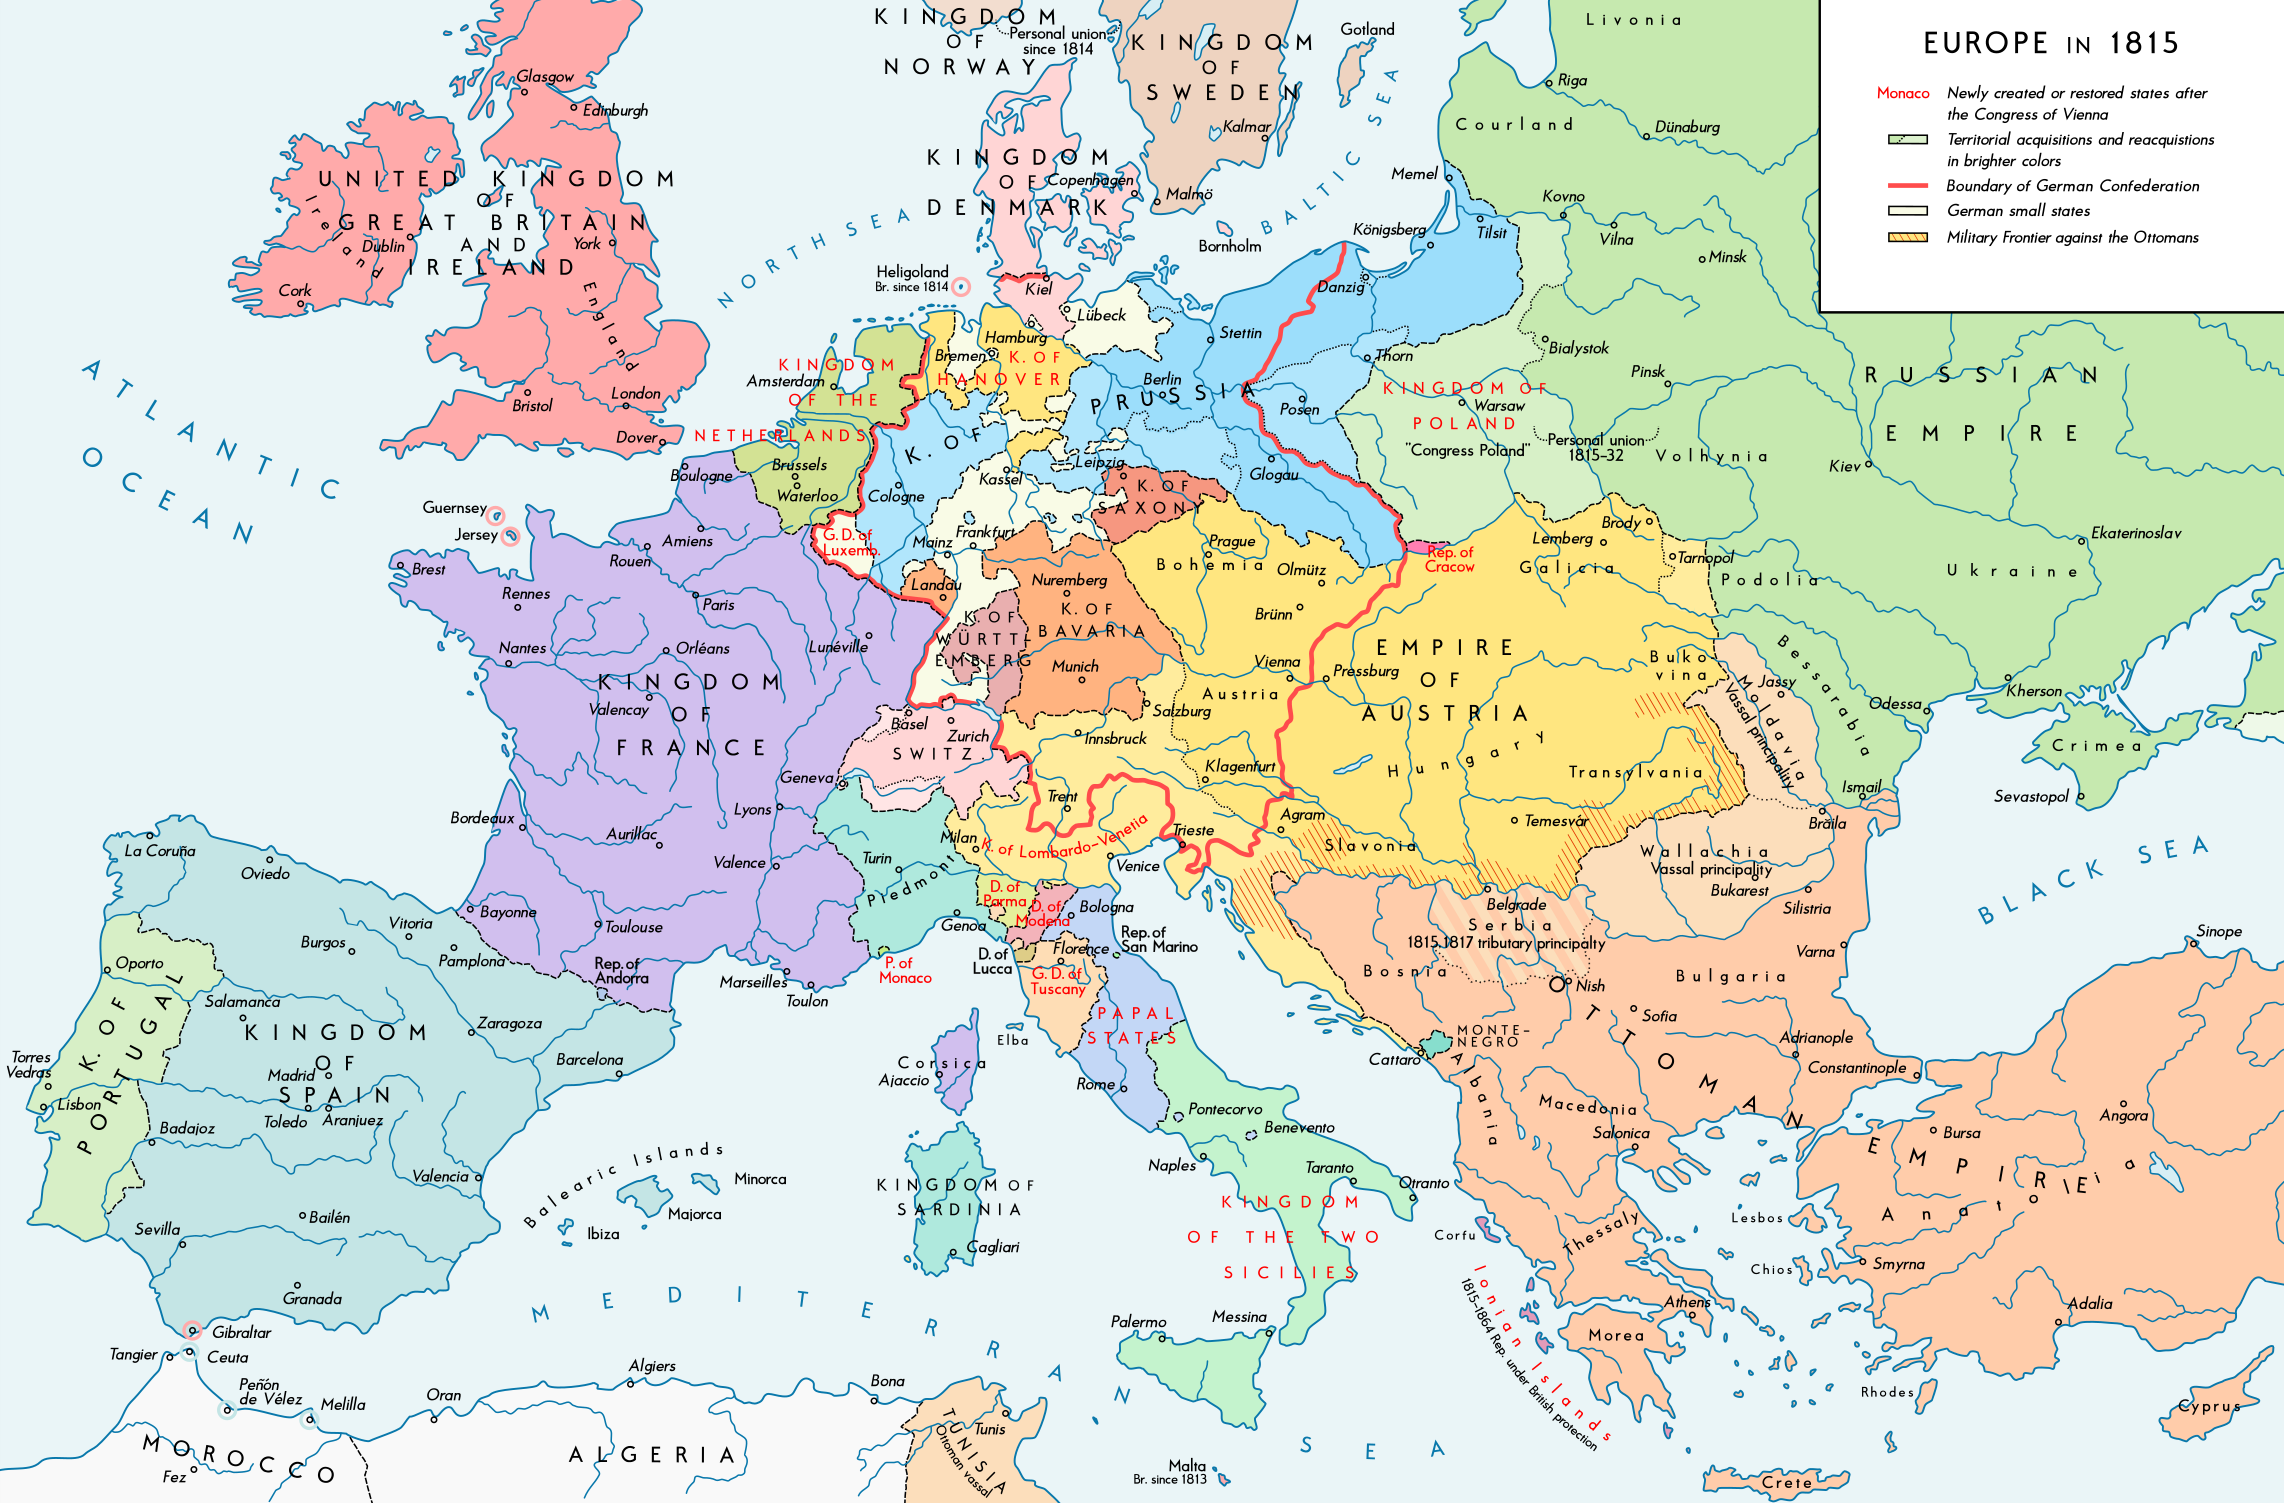
\includegraphics[width=\textwidth]{europe_congres_vienne.png}
	\caption{Les frontières de l'Europe redessinées en 1815 (Wikipedia)}
	\label{fig:my_label}
\end{figure}

\subsection{L'Italie}

Au début du 19\up{e}, la péninsule italienne est morcelée.
Le Nord est sous domination autrichienne, directement\footnote{La Lombardo-Vénétie fait partie des zones d'influence de l'Autriche.} ou indirectement\footnote{C'est le cas de la Toscane, de Parme, etc.}.
Seuls échappent à cette domination autrichienne les États de l'Église et le royaume de Piémont-Sardaigne.
\footnote{Rappelons-nous (cours d'introduction à l'histoire), au congrès de Vienne, on a fait des États tampons. Au Nord, c'est le royaume des Pays-Bas (amalgame de la Belgique et des Hollandais). Et au Sud-Est, le royaume de Piémont-Sardaigne.}
Ce royaume de Piémont-Sardaigne deviendra le moteur de l'unification italienne (à partir de 1848).

\subsubsection{Le \emph{Risorgimento} et le mouvement révolutionnaire de 1830 (Mazzini)}
%#39:34.9#

La vague révolutionnaire de 1830 manifeste des aspirations libérales (constitution) et nationales.
Ces deux aspirations, ce nationalisme de gauche, s'expriment dans  le mouvement du \emph{Risorgimento}.
C'est un mouvement intellectuel qui s’oppose au despotisme et à la domination autrichienne.

Le leader de ce mouvement est Giuseppe Mazzini.
Sous sa direction, un groupe de révolutionnaire entend chasser l’Autriche et établir une Italie républicaine et unitaire.
Notons que seulement 2\% de la population parle alors l’italien.
Les autres 98\% parlent des dialectes et ne se comprenne pas nécessairement.
C’est l’élite, répartie partout, qui se réclame du Risorgimento.
L’italien va se rependre petit à petit et devenir un moteur d’unité.
De son côté, en 1830 Mazzini multiplie en vain les tentatives d’insurrections.
C’est un échec.
L'explosion révolutionnaire de 1830 n'aboutit à rien, mais les idées font leur chemin.

Ainsi, en 1846, le pape Pie~IX est intronisé et il effectue une série de réformes comme la création d'un conseil d’état consultatif.
C’est un premier pas, timide, mais il donne de grands espoirs au gens du Risorgimento. 
Ce premier petite geste du pape, même modéré, donne l’exemple au roi de Piémont (Charles-Albert) puis au Grand-Duc de Toscane qui opèrent des réformes qui diminuent le despotisme.
Les idées libérales et nationales continuent à se développer et à prendre de l’importance dans toute la péninsule.

En conclusion, 1830 est un échec pour ce qui est de l'unification, mais les idées font leur chemin et portent des fruits à partir de 1846.

\subsubsection{La vague révolutionnaire de 1848}

Cette vague se situe dans un contexte de crise économique doublée d’une crise agricole. 
Le mouvement part, en Italie, de Sicile et se répand comme une trainé de poudre. 
En mars 1848, Charles-Albert puis le pape accordent des constitutions.

L’Autriche-Hongrie fait alors face à de graves troubles : le deuxième épicentre du printemps des peuples se situe à Vienne et le prince de Metternich doit fuir la capitale. 
Les patriotes italiens se tournent vers le roi du Piémont-Sardaigne mais Charles-Albert est réticent. 
Il a peur de faire le jeu des républicains car tous ces patriotes révolutionnaires ont des idées de plus en plus à gauche.
En plus, l’armée autrichienne reste puissante, même si Metternich a dû fuir.

Finalement, après hésitation, il se lance et déclare la guerre aux Autrichiens avec l’aide des révolutionnaires. 
Il délivre la Lombardie de la domination autrichienne. 
C’est une victoire mais les forces autrichiennes restent intactes et reculent. 
Quelques mois plus tard ces dernières repassent à l’offensive. 
En mars 1849, c’est le triomphe autrichien.

Charles-Albert abdique immédiatement en faveur de Victor-Emmanuel~II, son fils.
C’est un coup de maitre car de cette façon, il se plie devant la défaite mais maintient la dynastie à travers son fils. 
Ainsi, même vaincue, la dynastie piémontaise reste le symbole des nationalistes italiens. 
Il faut dire que les Français et les Anglais avaient fait pression pour que le Piémont reste intact et ne se fasse pas dévorer par l'Autriche.
\footnote{Ici, la France et la Grande Bretagne, en faisant pression pour que le Piémont-Sardaigne reste intact, jouent le jeu du congrès de Vienne, c'est-à-dire le jeu des équilibres : il faut que toutes les grandes puissances soient équilibrées. Il ne faut donc pas que l'Autriche s'agrandisse car sinon il faut aussi que la France et la Grande Bretagne puissent s'agrandir, etc.}

Le royaume de Piémont reste vraiment le seul espoir des patriotes italiens. 
Victor-Emmanuel~II, le nouveau roi, maintient sa constitution alors que partout ailleurs, les Autrichiens se lancent dans la répression\footnote{On appellera ça la seconde restauration, la première étant le congrès de Vienne.}.
À Rome, Pie~IX refuse toute autre réforme.
C'est ainsi que le royaume de Piémont-Sardaigne devient le moteur de l'unification italienne.

\subsubsection{Le royaume de Piémont-Sardaigne, moteur de l'unification (Cavour)}

%#3:28.9#

L’échec des révolutions de 1848 a montré aux patriotes italiens qu'ils doivent compter, d'une part sur un pouvoir fort capable d'organiser le peuple et de s'imposer aux princes, d'autre part sur une aide extérieure.
C'est la grande différence avec l'unification de l'Allemagne, où la Prusse fait tout toute seule.
Les Italiens comptent sur une aide extérieure.

Victor-Emmanuel~II, soutenu par Cavour\footnote{Camillo Cavour est, comme Mazzini, l'un des personnages principaux du Risorgimento. C'est une nouvelle génération : il y avait le roi Charles-Albert et Mazzini, maintenant, il y a Victor-emmanuel~II et Mazzini.}, entend jouer ce rôle de pouvoir fort.
Cavour est un anticlérical modéré et réaliste, beaucoup plus à droite que Mazzini qui était républicain et démocrate.
Il entend, lui aussi, chasser les Autrichiens de la péninsule italienne.

Cavour commence par moderniser le royaume de Piémont pour que ce soit un pôle d’attraction politique et économique\footnote{Il modernise l'État de Piémont-Sardaigne, mais aussi son économie.} pour toute la péninsule. 
Puis, à partir de 1850, il encourage, partout dans la péninsule, les foyers révolutionnaires (les patriotes\footnote{Patriotes clandestins, puisque la répression s'est abattue après 1848.}). 

\subsubsection{La question italienne sur la scène internationale (1850-1870)}

%#4:39.5#

Ensuite, Cavour porte la question italienne sur la scène internationale. 
Il a conscience qu’il ne fera jamais l’unification sans aide extérieur.
Il attire le soutien de la Grande Bretagne et de la France de Napoléon~III en participant à la guerre de Crimée contre la Russie en 1854 et 1855.
\footnote{La Russie veut avoir un accès à la mer par le sud et s'oppose à l'Empire ottoman. La France et la Grande Bretagne s'opposent à cette extension de la Russie. Le Piémont-Sardaigne leur apporte ainsi une petite aide pour s'attirer leurs bonnes grâces.}

Face à cette aide, Napoléon~III hésite à soutenir Cavour dans une guerre contre l’Autriche.
Comment souvent, Napoléon~III, en essayant de ne s’aliéner personne, s’aliéna tout le monde : l’Autriche est catholique, or il ne veut pas se mettre à dos les catholiques français qui sont pour le pape, et en plus les hommes d’affaires veulent la paix, etc.

Finalement, en 1858, Napoléon~III fait un accord avec Cavour.
Il n’est pas satisfaisant, mais Cavour y voit une première étape. 
Le Piémont arrache la Lombardie-Vénétie et la Savoie-Nice à l’Autriche, et l'accord promet que la France reçoive la Savoie-Nice.
Les États pontificaux sont préservés (concessions de Cavour).
Napoléon se dit satisfait et va soutenir les Italiens.

Fort de cet accord, en 1859, Cavour multiplie les provocations vis-à-vis de l’Autriche.
L’Autriche entre en guerre : ce sont les fameuses batailles de Magenta et Solferino en 1859.\footnote{Ces batailles sont importantes. 1859 est \emph{une date à retenir}. La bataille de Solferino est assez connue, parce qu'il y a alors un médecin suisse, Henry Dunant qui est effaré de ce qu'il observe. Il se rend compte que la majorité des soldats qui meurent sur le champ de bataille décèdent lamentablement par manque de soin. C'est ainsi qu'il crée la Croix-Rouge et que sont promulgués, en 1864, les accords de Genève. Ce sont les lois de la guerre qui concernent les trèves des brancardiers, l'aide aux blessés, etc. sur les champs de bataille.}
Il y a eu \numprint{30000} morts à Magenta et \numprint{40000} à Solferino.
Ces deux batailles sont des victoires française et piémontaise contre les Autrichiens.

Napoléon~III, effrayé comme à son habitude, ne veut pas aller trop loin et signe alors la paix avec les accords de Zurich.
Dans cette paix, la France obtient bien la Savoie-Nice, mais le Piémont obtient la Lombardie sans la Vénétie\footnote{Ils voulaient la Lombardo-Vénétie (cf. les accords entre le Piémont et la France).}, qui reste autrichienne.
Cela déclenche évidemment la colère des patriotes italiens contre Napoléon~III qui, face à cette colère, commence petit à petit à se rendre compte que l'idée de démembrer les États Pontificaux est inéluctable.

Pour continuer l'unification au sud, Cavour utilise ensuite les forces révolutionnaires de Garibaldi\footnote{Giuseppe Garibaldi (1807--1882) est un personnage fondamental du Risorgimento italien, pour avoir personnellement conduit et combattu dans un grand nombre de campagnes militaires qui ont permis la constitution de l’Italie unifiée. Il a essayé, le plus souvent, d’agir sous l’investiture d’un pouvoir légitime, ce qui ne fait pas de lui à proprement parler un révolutionnaire (Wikipedia). Déjà après la répression de 1848, Garibaldi avait lutté pour le gouvernement provisoire de Milan, puis s'était rattaché à la monarchie de Victor-Emmanuel~II.} pour prendre le royaume de Naples.
Ce dernier prend donc tout le Sud, et le remet à la monarchie piémontaise.
Cavour s’inquiète ensuite de la puissance de Garibaldi qui remonte vers le nord.
Il convainc les Français d’arrêter Garibaldi à Rome. Évidemment, ces derniers sont d'accord et la protègent.
Garibaldi tente en effet de prendre Rome, mais c'est un échec.

En 1861, Cavour meurt en disant : \enquote{l’Italie est faite.}
Il n’est pas loin de la vérité même si l’Italie n’est pas tout à fait faite : il manque la Vénétie et Rome. 
La Vénétie revient finalement à l’Italie cinq ans plus tard, par le biais de l’unification allemande après la défaite autrichienne contre la Prusse à Sadowa en 1866. 
Pour le prix du silence de la France, la Prusse offre la Vénétie à la France qui la donne à l’Italie.

Rome, elle, reste protégée par les Français.
En 1867, Garibaldi tente une insurrection à Rome, mais c'est de nouveau un échec.
Il faut attendre la défaite française contre les Prussiens à Sedan en 1870 pour prendre le territoire des États pontificaux (sauf le Vatican), et pour Rome puisse être proclamée capitale de l'Italie.
Cependant, la question du pouvoir du pape reste un problème : il y aura des tensions entre le Vatican et le Quirinal\footnote{Lieu de résidence papale puis présidentielle.} jusqu'en 1929 avec les accords du Lantran entre Mussolini et le pape.
\footnote{Les accords du Latran, c'est : réduction du pouvoir du pape au tout petit territoire du Vatican, mais le catholicisme redevient religion d'État en Italie.}

\subsection{L'Allemagne}

%#12:00.9#

Cette unification se fait différemment de l’Italie, et pour comprendre l'unification de l'Italie, il faut comprendre celle de l'Allemagne.
En Italie, c'est une unification dont la volonté vient du bas, encadrée par le haut, et pour laquelle il y a une aide internationale.
Du côté allemand, c'est le contraire. Cela vient d'en haut. Le moteur est la Prusse, qui n'a qu'un souci : que les autres puissances la laissent faire. Elle ne demande aucune aide.

Les vagues de 1830 et 1848 consacrent la défaite des libéraux en Prusse et laissent donc le champ libre aux conservateurs sur lesquels s’appuient la dynastie prussienne des Hohenzollern. 
Le roi de Prusse est alors Guillaume~I\up{er} et son chancelier est Otto von Bismarck
Otto déteste le libéralisme mais il est d’un grand réalisme politique car il s'appuie sur les libéraux quand c'est nécessaire.
Ils veulent tous deux fonder un empire sur l’adhésion des princes\footnote{Roi de Bavière, duc de Wurtemberg, etc.} et non celles des peuples (cf. différence avec l'Italie).
L’unification sera prussienne, conservatrice, autoritaire et antiautrichienne. 

La Prusse a alors une constitution conservatrice. 
Certes, on a un parlement, mais les ministres ne sont pas responsables devant ce parlement.
Ils sont nommés par le roi et responsables devant le roi.
Le roi peut donc défaire ses ministres quand il le souhaite, ou garder un ministre/chancelier même s'il perd les élections.
C'est ainsi qu'on peut expliquer la longévité de Bismarck comme chancelier : Guillaume le nomme chancelier pour écraser les libéraux\footnote{Les libéraux représentaient une difficulté pour la réalisation de l'unification telle que voulue par Guillaume et Bismarck.}, et choisit de le laisser à ce poste durant tout son règne.
Bismarck ne sera congédié que par le successeur de Guillaume : Guillaume~II.

%L’adhésion des princes ne va pas de soi. 
%Le roi de Bavière est important et il y a beaucoup des princes puissants pas faciles à dominer.



\subsubsection{La prospérité prussienne}

De 1850 à 1862, la Prusse connait un formidable essor économique.
\footnote{Elle enclenche sur la première révolution industrielle qui avait débarqué en Belgique sur le continent européen. La révolution industrielle commence toujours difficilement, c'est une période de dépression : il faut des capitaux, il y a des outils qui changent, etc. Mais à partir de 1850, de manière générale en Europe et particulièrement en Prusse, c'est un essor économique extraordinaire.}
En 1834, c'est le Zollverein : une union douanière et économique entre les États allemands.
L'Autriche est un empire "snob", et elle refuse d'entrer dans cette union douanière où elle n'a pas un rôle prépondérant.

L’Autriche commet ainsi une erreur monumentale en ne rejoignant pas cet accord. 
Cet accord unifie économiquement l'Allemagne avant qu'elle ne soit unifiée politiquement.
On l'observe à travers la construction du chemin de fer.
\footnote{La première révolution industrielle, c'est le textile, avec métier à tisser, mais c'est surtout les trains.}
On voit qu'à partir de 1850, l'Allemagne est unifiée économiquement par les trains.
La production de charbon est la deuxième du monde.
De grandes industries (notamment les usines Krupp) apparaissent dans la Ruhr, qui restera le poumon économique de l'Allemange jusqu'à la deuxième moitié du 20\up{e} siècle.

\subsubsection{Bismarck et l'unification par les guerres (les duchés, Sadowa, Sedan)}

Le chancellier a bien compris que, pour que l'unification se fasse sous l'égide de la Prusse, il faut d'abord éliminer l'influence autrichienne.
Il faut donc en premier lieu abattre l'Autriche (par les armes) et, pour cela, obtenir la neutralité de la Russie et de la France.
\footnote{Noter que Bismarck ne veut pas que la Russie et la France soient des alliés, mais il veut simplement faire en sorte que ces pays n'interviennent pas pour venir en aide à l'Autriche.}

Pour amadouer la Russie, Bismarck envoie des renforts aux troupes du tsar pour écraser les révoltes de Pologne en 1863.
La Pologne essaye d’exister mais est à chaque fois réprimée.
Les Polonais avaient déjà été écrasés en 1830 et ils le sont à nouveau en 1863.

Pour s'attirer la neutralité de la France, le chancellier berce Napoléon~III en lui chantant la comptine de la Belgique.
Napoléon~III est une menace pour l'existence de la Belgique : il rêve d'annexer ces territoires.
\footnote{La France avait perdu beaucoup de territoire (notamment au profit de la Belgique). Napoléon~III lorgne sur ces territoires perdus.}
Bismarck le laisse doucement rêver en lui laissant miroiter une révision du traité du congrès de Vienne.

% #19:34.5#

\section{La Commune de Paris, 1871}

\subsection{Les origines lointaines}

\subsubsection{Transformation de Paris}

\subsubsection{Réveil de l'agitation ouvrière}

\subsection{Les origines prochaines}

\subsubsection{Chute du Second Empire}

\subsubsection{Divorce entre Paris et la province}

\subsection{Le déroulement}

\subsection{Les significations}


\chapter{Les développements économiques et sociaux au XIX\up{e} siècle}

\section{La première révolution industrielle, 1815-1871}

\subsection{Évolution de la conjoncture économique}

\subsubsection{La période 1820-1850}

\subsubsection{La période 1850-1870}

\subsection{Transformations sociales et stéréotypes sociaux}

\subsubsection{Le modèle bourgeois}

\subsubsection{La figure de l'ouvrier}

\section{La deuxième révolution industrielle, 1871-1914}

\subsection{Évolution de la conjoncture}

\subsubsection{La crise de 1873-1894}

\subsubsection{La reprise économique de la Belle Époque}

\subsection{Le Darwinisme social (rappel : scientisme)}

\subsection{Les difficiles conquêtes du monde ouvrier : le cas de la Belgique}

\subsubsection{Les grêves de 1886}

\subsubsection{La nécessité de légiférer}

\section{L'expansion coloniale}

\subsection{L'ampleur du mouvement}

\subsection{Mobiles de l'expansion coloniale}

\subsubsection{L'explication économique}

\subsubsection{L'explication politique}

\subsubsection{Les faits : la Tunisie et l'Égypte}




\part{Le XX\up{e} siècle}

\chapter{Le nationalisme}

\section{La conception germanique}

\section{La conception latine}

\section{Une évolution complexe : le culte de la Patrie}


\chapter{La Première Guerre mondiale}

\section*{Introduction (débats historiographiques)}

\subsection{Les entrées en guerre}

\subsection{Le consentement à la guerre longue : le cas de la Belgique}

\subsection{Le viol de la neutralité et l'invasion}

\subsection{Les massacres de civils}

\subsection{Le front}

\subsection{La Belgique occupée}

\section{Les mémoires de guerre (héroïsation et stigmatisation)}

\section{La démobilisation des esprits}

\chapter{Les transformations économiques et sociales}

\section{Sortir de la grande guerre et reconstruire}

\section{L'Occupation de la Ruhr, 1923}

\section{La crise de 1929 et ses conséquences (rappel)}

\chapter{Les totalitarismes (fascisme et communisme)}

\section{Le Fascisme italien}

\subsection{Les caractéristiques du système}

«~Tout dans l’Etat, rien contre l’Etat, rien en dehors de l’Etat~» (Mussolini)

«~Je prends l’homme au berceau et je ne le rends au Pape qu’après sa mort~» (idem)

\subsection{Bilan du fascisme}

\subsubsection{Au niveau démographique}

\subsubsection{Au niveau économique}

\subsubsection{Au niveau social}

\subsubsection{Au niveau religieux}

\subsubsection{Au niveau culturel}

\section{Le National-Socialisme allemand}

\subsection{Le parti national-socialiste des travailleurs allemands}

\subsection{Les caractéristiques du système nazi}

- L’idéologie est décrite dans Mein Kampf (1925-1926).
- L’Etat raciste est au service d’une politique de la race

\subsection{L'hitlérisme en pratique}

\subsubsection{Un pouvoir fasciste}

- Centralisation du pouvoir
- Mobilisation idéologique
- Instauration d’un régime corporatiste
- La remise en ordre de l’économie

\subsubsection{Un pouvoir raciste}

\section{Le Stalinisme}

\subsection{Le triomphe idéologique}

\subsection{La centralisation du pouvoir et les pratiques de terreur}



\chapter{La Deuxième Guerre mondiale}

\section{Les origines du conflit}

\subsection{L'ombre portée de la Grande Guerre}

\subsection{La politique internationale et militaire allemande}

\section{La guerre 1940-45}

\subsection{Les opérations militaires}

\subsection{Les occupations}

\subsection{Les résistances et les collaborations}

\section{sortir de la guerre}

\subsection{La remise en place de l'État (rappel)}

\subsection{Les répressions des collaborations}

\subsection{Les mémoires de guerre}


\chapter{La construction européenne}

\section*{Introduction : l'héritage de la guerre (mémoire et pardon)}

\section{La coopération européenne intergouvernementale}

\subsection{Les organisations à caractère économique}

\subsection{Une organisation à caractère politique}

\section{Vers l'intégration : de la CECA (1951) à Maastricht (1992)}

\subsection{Les Utopies fondatrices (1940-1947)}

\subsection{La mise en route de l'Europe des six}

\subsection{La parenthèse De Gaulle (1963-1969)}

\subsection{L'élargissement de la CEE}

\subsection{Quelques critiques adressées à la CE}


\chapter{Les décolonisations}

\section*{Introduction}

\section{Les causes de la décolonisation}

\subsection{Les sources de mécontentement}

\subsection{Les conséquences de la Deuxième guerre mondiale}

\subsection{Un environnement international favorable}

\section{La décolonisation de l'Asie}

\subsection{Les métropoles face à la décolonisation}

\subsection{La décolonisation négociée}

\subsection{La décolonisation violente}

\section{La décolonisation de l'Afrique}

\subsection{L'Afrique du Nord}

\subsection{L'Afrique noire}


\part*{Conclusion}



\end{document}
